\chapter[General Introduction]{General Introduction}
\label{chapter_1}

%% The following annotation is customary for chapter which have already been
%% published as a paper.
%\blfootnote{Parts of this chapter have been published in Annalen der Physik \textbf{324}, 289 (1906) .}
%
%%% It is only necessary to list the authors if multiple people contributed
%%% significantly to the chapter.
%\authors{Albert {\titleshape Einstein}}
%
%%% The '0pt' option ensures that no extra vertical space follows this epigraph,
%%% since there is another epigraph after it.
%\epigraph[0pt]{
%    Nature and nature's laws lay hid in the night; \\
%    God said `Let Newton be!' and all was light.
%}{Alexander Pope}
%
%\epigraph{
%    It did not last: the devil shouting `Ho. \\
%    Let Einstein be!' restore the status quo.
%}{Sir John Collings Squire}

\begin{abstract}
	In this chapter I present a general introduction to the thesis. While the main interest is to understand the mechanism by which the nuclear pores in our cells operate, various topics and techniques are touched upon. Starting from a brief overview of the cellular organization, I narrow down into the nuclear pore complex, from the first discoveries of its architecture and composition to recent theories describing how nuclear transport is regulated. Furthermore, I discuss the importance of biomimetic approaches to study nuclear transport, with a particular emphasis on solid-state-nanopore and DNA-origami technologies.
\end{abstract}

\newpage
\section[Introduction]{Introduction}
\sectionmark{Chapter 1}
Life on earth is extremely diverse and variegated, from single-cell entities like  bacteria or yeast, to complex multi-tissue organisms such as humans. To achieve the sophistication found in more complex systems like eukaryotes, molecules are organized into organelles which, just like the organs in our body, carry out different specialized tasks (Figure \ref{fig:fig1.1}a) \cite{Lodish2000}. For example, mitochondria produce the chemical energy needed to perform biochemical reactions in the cell, ribosomes read strings of mRNA to synthesize new proteins, while the nucleus stores the hereditary information in the form of DNA\cite{Nelson2008}. To safely protect the genetic material, eukaryotic cells feature a double membrane nuclear envelope (NE) that encloses and physically isolates the nucleus from the rest of the cell \cite{Hetzer2010}.
%The presence of membrane-divided cellular compartments necessitates efficient communication pathways that regulate the exchange of material across the membrane. 

Nuclear Pore Complexes (NPCs) are large protein assemblies that form $\sim$40nm-wide channels across the NE and behave as gatekeepers by controlling the trafficking of RNAs, proteins, and metabolites between the nucleus and the cytoplasm (Fig.\ref{fig:fig1.1}b) \cite{Wente2010}. In a single cell, the number of nuclear pores can vary  from 75–150 in a yeast cell \cite{Winey1997} to $\sim$3000-5000 pores in a human cell \cite{Gorlich1999}, to $\sim5\times 10^7$ in a mature \emph{Xenopus} oocyte \cite{Cordes1995}. A fascinating aspect of the NPC is its unique combination of high versatility while retaining specificity. In fact, up to 30 different types of transporter proteins are recognized and allowed to efficiently translocate through the NPC, while precluding the transport to all other large molecules \cite{Mackmull2017}. The secret for such highly selective transport relies in a group of key proteins, called FG-Nups, which form a tangled spaghetti-like mesh within the central channel of the NPC \cite{Wente2000}. 

%Different cell types exist such as neurons, muscle cells, or white blood cells, which carry out diverse functions in our body, yet they are all built from the same fundamental molecules, such as nucleic acids (DNA and RNA), proteins, and lipids, and carbohydrates . To achieve their functional diversity and complexity, molecules in eukaryotic  cells are arranged into isolated organelles where, just like the organs in our body, carry out different specialized tasks (Figure \ref{fig:fig1.1}a). For example, mitochondria produce the chemical energy needed to perform biochemical reactions in the cell, ribosomes read strings of mRNA to synthesize new proteins, while the nucleus stores the hereditary information in the form of DNA\cite{Nelson2008}. Unlike for prokaryotes, where there is no membrane-bound nucleus, eukaryotic cells feature a double membrane nuclear envelope (NE) that safely encloses and segregates the genetic material from the rest of the cell \cite{Hetzer2010}. Such compartmentalization is employed by eukaryotic cells, such as human cells, for efficiency purposes since it allows to independently tune the microenvironment of the different organelles to better perform their task.



\begin{figure}[!htbp]
	\centering
	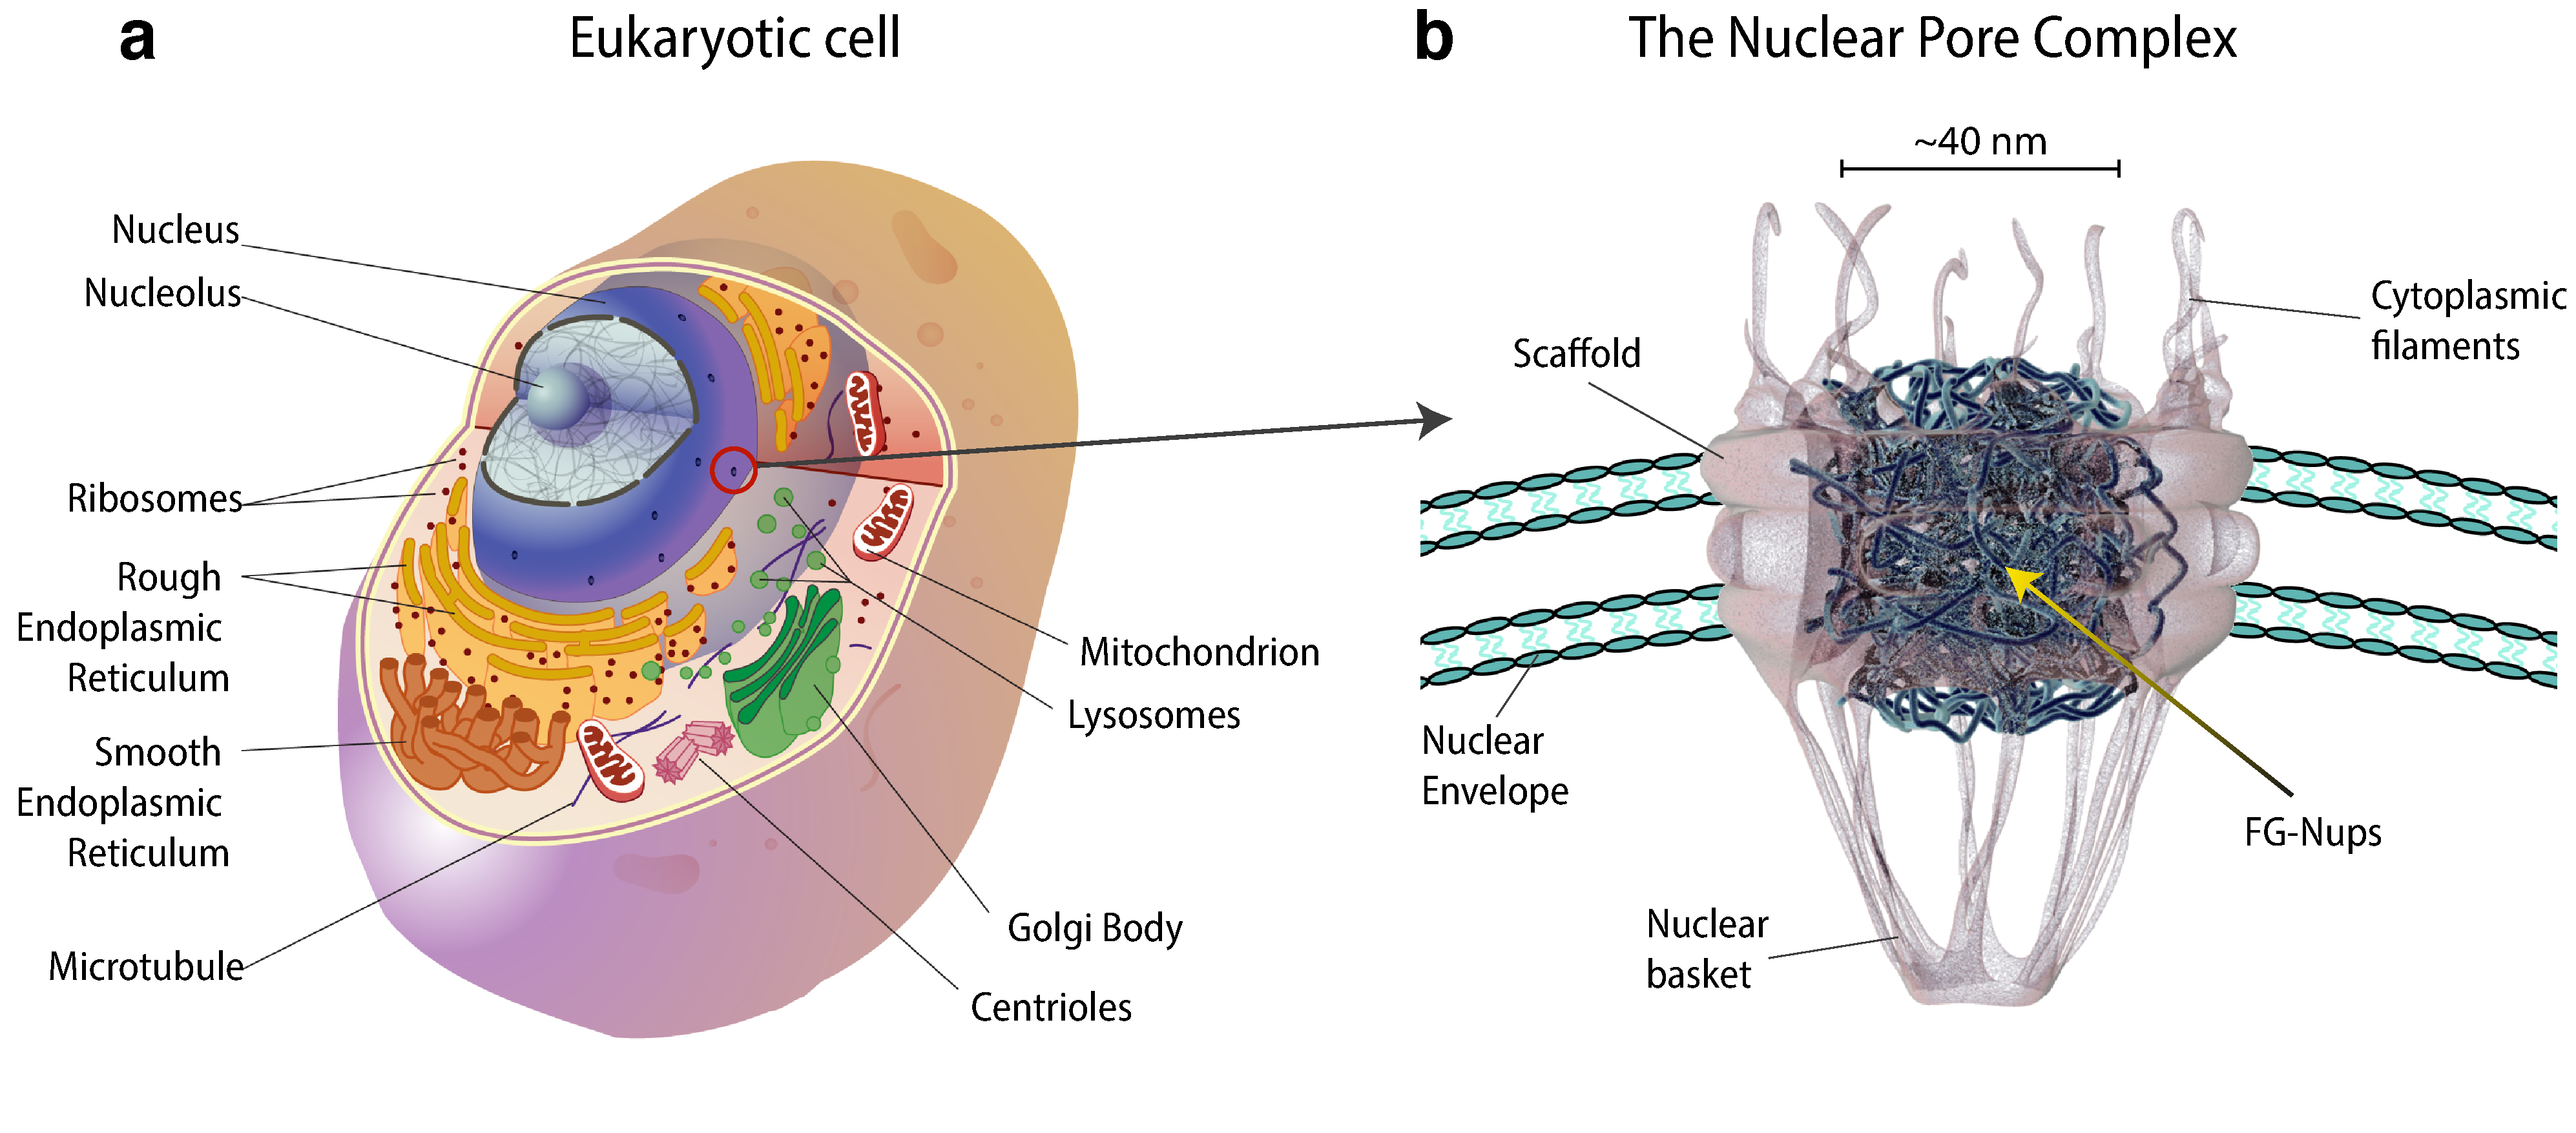
\includegraphics[width=1\linewidth]{figures/Figure1.1.pdf}
	\caption{a, Schematic of an eukaryotic cell, adapted from \cite{url:https://www.genome.gov/genetics-glossary/Organelle}. b, Illustration of the nuclear pore complex embedded in the nuclear envelope. FG-Nups (blue) line the central channel forming a spaghetti-like mesh. Adapted from a design of Samir Patel.}
	\label{fig:fig1.1}
\end{figure}


\noindent In this thesis, we work towards understanding the physical principles underlying this remarkable NPC selectivity, leveraging on techniques from molecular biology to nanotechnology. To understand and properly interpret the signal coming from our nanodevices, we first delve into a physical characterization of the noise sources that affect ion current measurements in solid-state nanopores. We then move on to engineer a fully synthetic FG-Nup from scratch and study its selective properties by reconstituting an artificial mimic of the NPC transport barrier using such a designer protein. Additionally, we provide supporting evidence that point to a mechanistic description of nuclear transport by studying the behavior of a purified native FG-Nup. Finally, we take a major step towards the reconstitution of an artificial nucleus by embedding 30nm-wide DNA-origami pores into the membrane of a lipid vesicle. The present work opens the way to multiple exciting applications and follow-up projects towards the recapitulation and physical understanding of nuclear transport, as well as creating artificial models of the nucleus that can be employed in synthetic cells.

\section{The nuclear pore complex}
%\sectionmark{Chapter 1}
\subsection{Architecture and composition}
First evidence of the existence of the NE and nuclear pores was provided in 1950 by Callan and Tomlin \cite{CALLAN1950}, who performed imaging of the nuclear membrane of oocytes from amphibia using electron microscopy (EM). 
Further investigation by Gall in 1967 \cite{Gall1967} revealed the octagonal symmetry of nuclear pores (Figure \ref{fig:fig1.2}a,b), which was confirmed by other follow-up studies \cite{Aaronson1974,Franke1970}. Further refinements of the NPC structure using EM allowed to resolve other peripheral parts of the NPC, which include the cytoplasmic filaments and nuclear basket (Fig.\ref{fig:fig1.2}c–e, [refs]) \cite{Goldberg1999,Pante1996}. The biochemical composition of the NPC consists of $\sim$30 different types of nucleoporins (Nups) repeated in multiple copies following the octagonal symmetry of the pore. The distribution of Nups is modular and they can be distinguished in three categories \cite{Devos2006,Onischenko2017}: (1)  transmembrane Nups that anchor the NPC to the NE; (2) scaffold Nups that
\begin{figure}[!hbp]
	\centering
	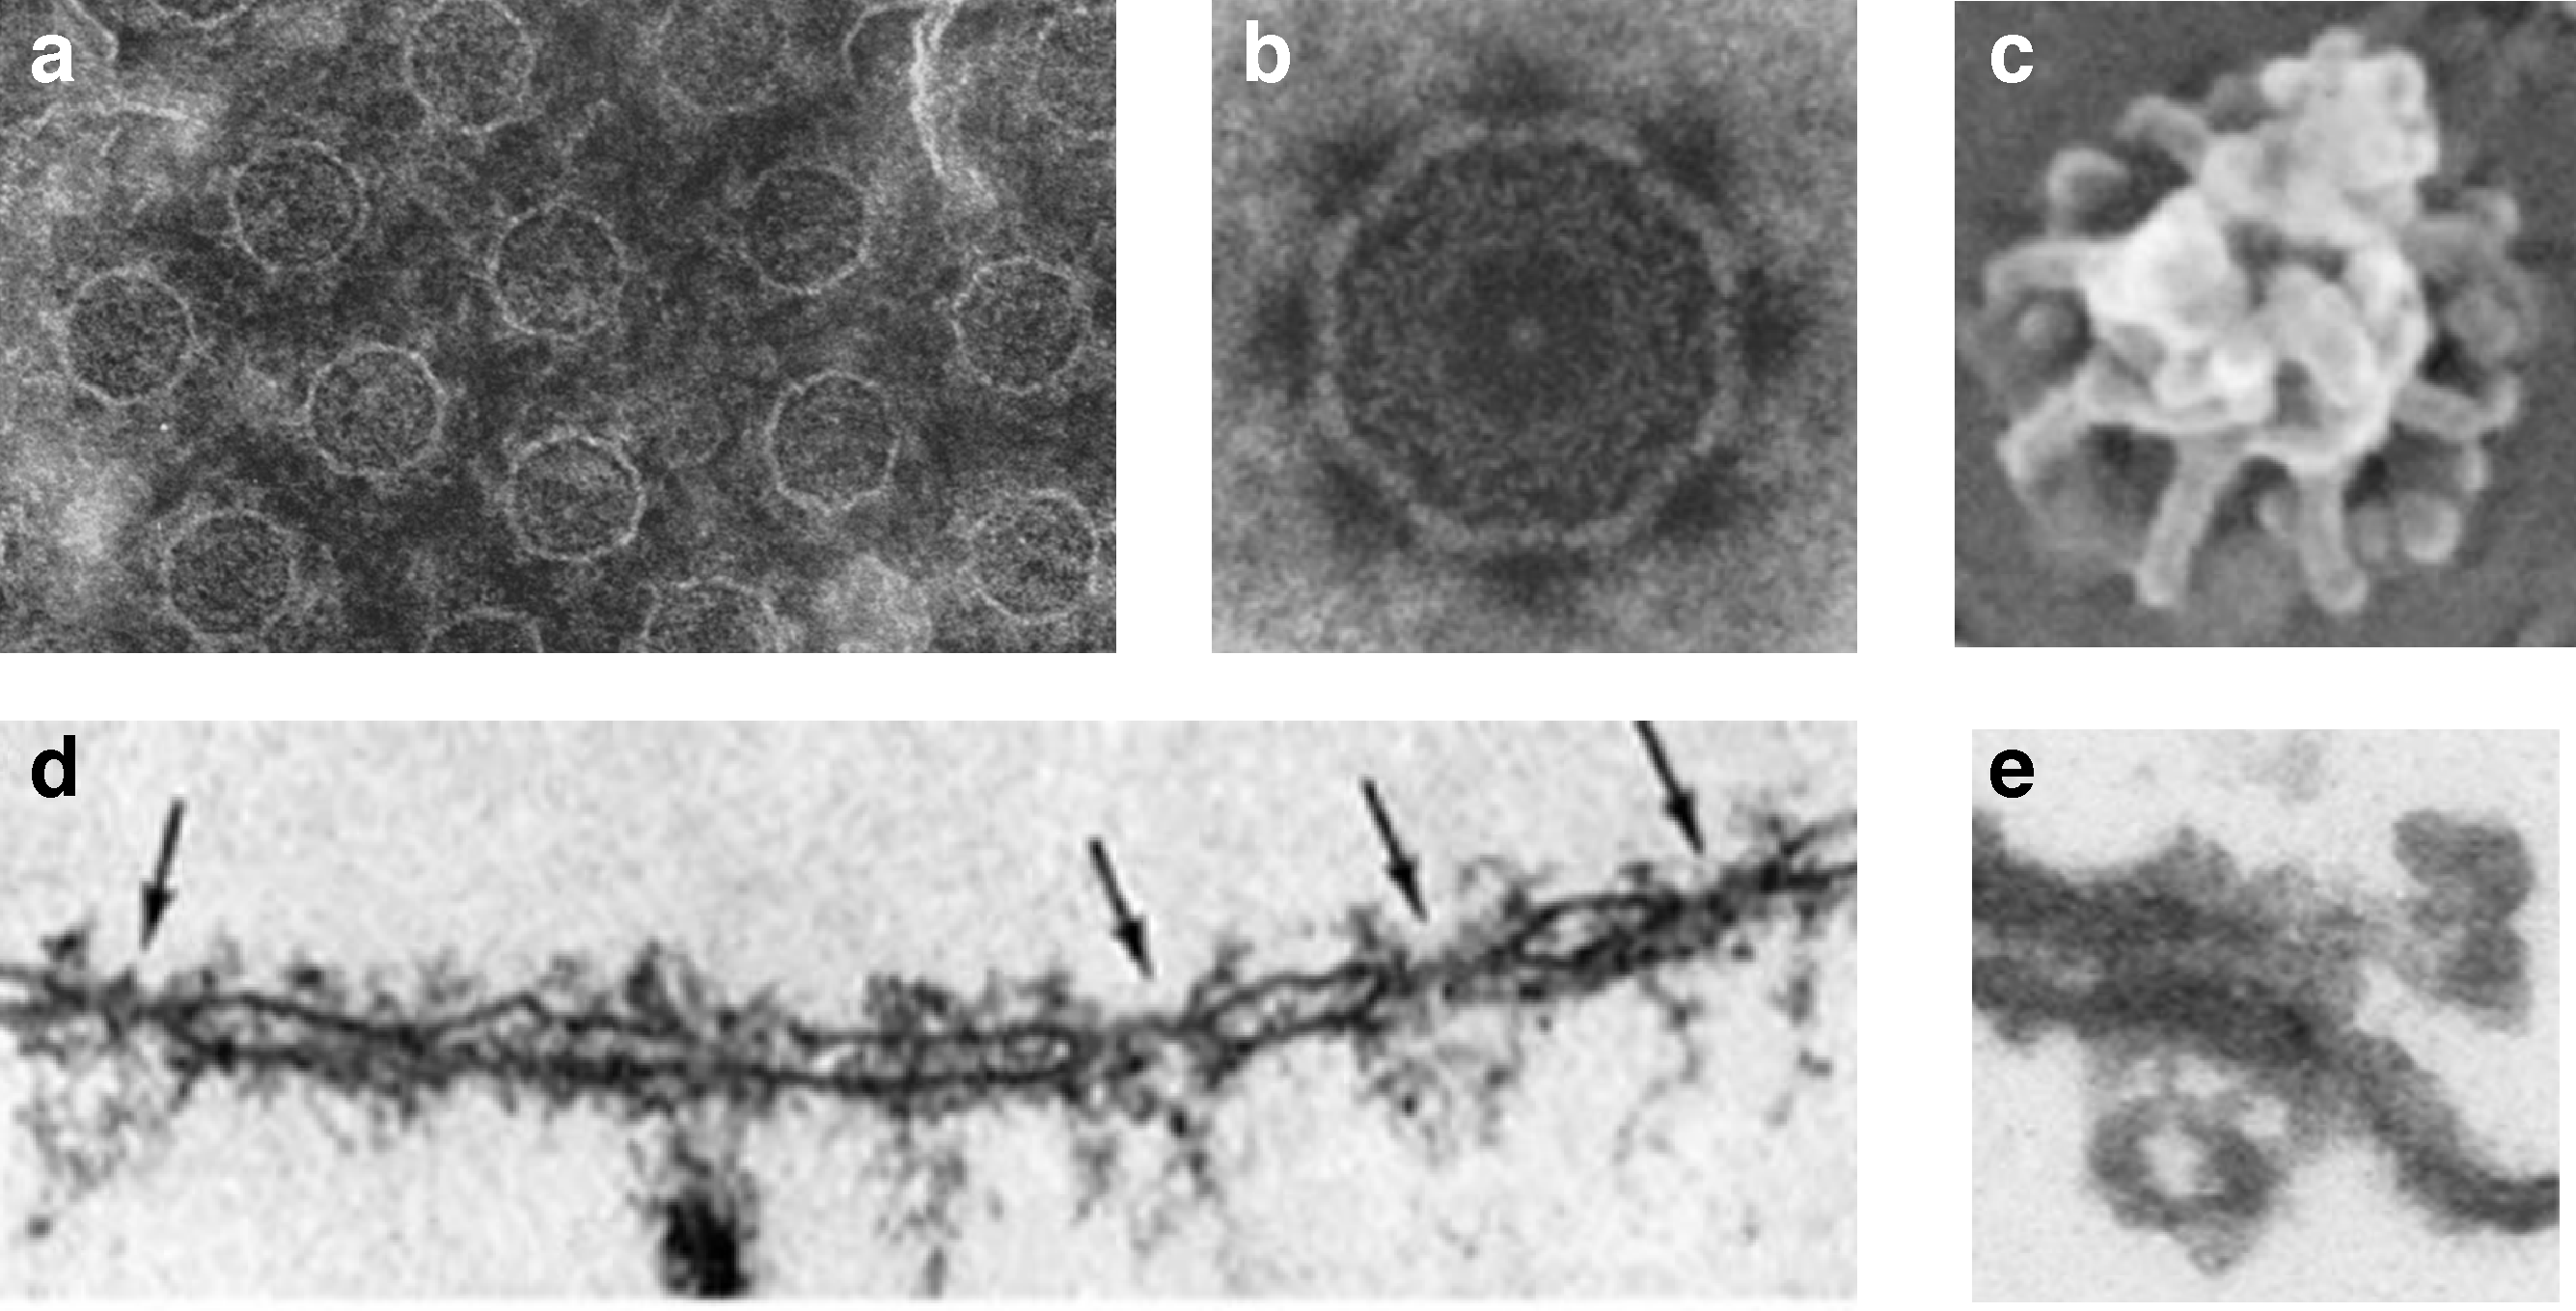
\includegraphics[width=1\linewidth]{figures/Figure1.2.pdf}
	\caption{a,b, Negative staining EM showing octagonal cross-sections of nuclear pore complexes extracted from Triturus alpestrus nuclei (adapted from \cite{Gall1967}). c, Electron microscopy structure of the nuclear pore complex from the nucleoplasmic side. Adapted from \cite{Goldberg1999}. d,  Negative staining EM of the nuclear envelope featuring embedded NPCs (pointed by arrows). Adapted from \cite{Pante1996}). e, Transmission electron microscopy image of a nuclear pore complex. Adapted from \cite{Lim2008}.}
	\label{fig:fig1.2}
\end{figure}
form a rigid ring-like structure to which intrinsically disordered (3) FG-Nups, rich in tandem ‘Phenylalanine-Glycine’ (FG) repeats, are anchored by their C-terminal domain and fill up the NPC central channel forming a gel-like mesh. 


\subsection{FG-Nups – types and motifs}
The central channel of the NPC is lined with intrinsically disordered FG-Nups (11 different types in yeast \cite{Yamada2010}). Based on their amino-acid sequence, FG-Nups appear quite redundant, with all of them featuring tandem Phe-Gly (FG) repeats separated by spacer sequences of $\sim$5-20 amino-acids (Fig.\ref{fig:fig1.3}a) \cite{Terry2009}. Moreover,  they are evolutionary conserved in their overall composition and structure \cite{Peyro2015}. FG-Nups can be broadly divided into two main categories \cite{Yamada2010,Terry2009}: (1) FXFG-Nups which are abundant in Phe-Any-Phe-Gly (FXFG) repeats, where ‘X’ can be any amino-acid, featuring spacers relatively high in charge ($\sim$26-36\% of amino-acids has a charge), which confer FXFG-Nups with an overall extended and dynamic conformation; (2) GLFG-Nups that instead are rich in Gly-Leu-Phe-Gly (GLFG) repeats with spacer sequences enriched in ‘Q’ and ‘N’ amino-acids. Unlike FXFG-Nups, these possess a low amount of charged amino-acids (2-3\%) resulting in a more collapsed coil configuration. Strikingly, deletion of all FG-Nups other than the GLFG-Nups Nup100, Nup116, and Nup145, was shown to still support efficient nuclear transport \emph{in vivo} without impairing the viability of the cell, which showcases the outstanding robustness and redundancy of the FG-Nup barrier \cite{Adams2016}.
\begin{figure}[!htbp]
	\centering
	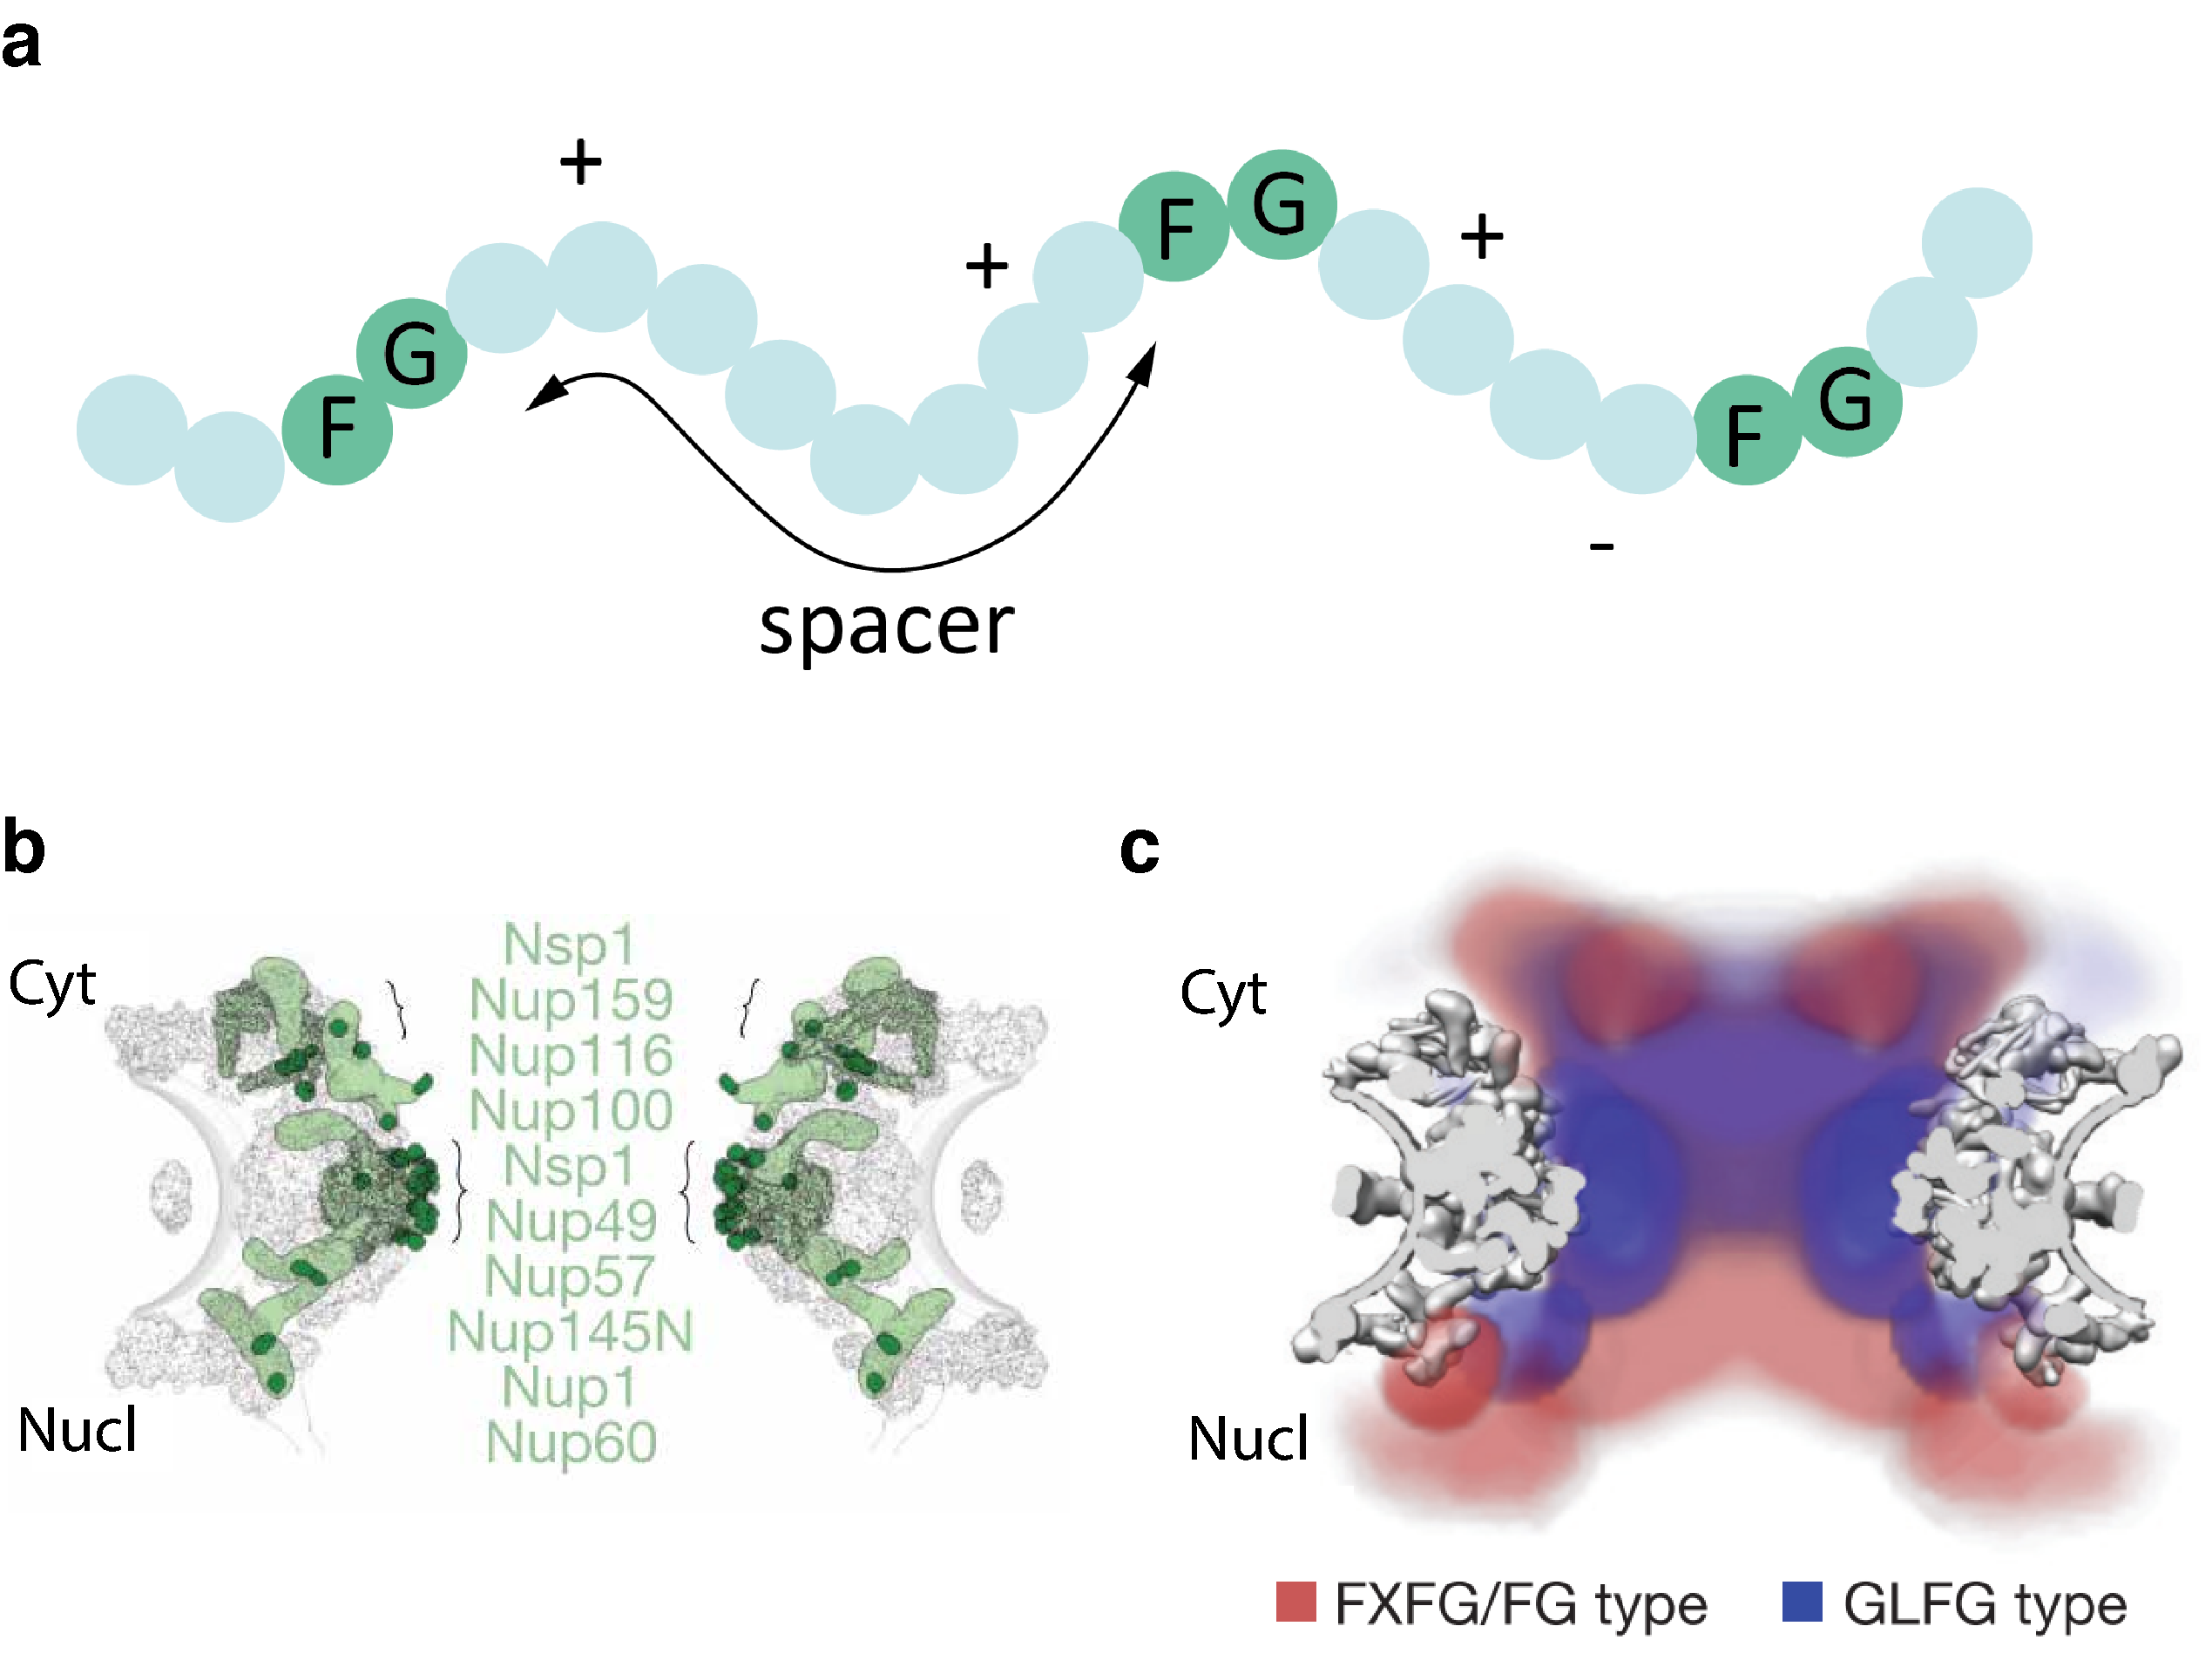
\includegraphics[width=0.85\linewidth]{figures/Figure1.3.pdf}
	\caption{a, Representation of a characteristic FG-Nup protein sequence. b, Structure of the NPC scaffold (grey) with highlighted FG-Nups anchor domains (light green) and FG-repeat emanating points (dark green). c, Heat map of the GLFG (purple) and FXFG (red) domains from Brownian dynamics simulations. b and c were adapted from \cite{Kim2018}.}
	\label{fig:fig1.3}
\end{figure}

\subsection{Nucleocytoplasmic transport}	
FG-Nups are key players in regulating molecular transport across the NE \cite{Wente2000}. While allowing the passive diffusion of small molecules, \emph{e.g.} water, ions, and proteins up to a size cut-off of $\sim$40 kDa, transport of large molecules (>40 kDa) occurs selectively \cite{Zilman2007}: inert macromolecules are hindered by the FG-mesh unless they are bound to a nuclear transport receptor (NTR). Karyopherins (or Kaps) constitute the largest family of NTRs \cite{Tu2011}, with importin-$\beta$ (Imp$\beta$, Kap95 in yeast) being the most characterized as it plays a central role in nuclear import \cite{Harel2004}. It features $\sim$9-10 hydrophobic pockets on its convex surface that can specifically bind FG-motifs \cite{Bayliss2000}, which in turn facilitates its partitioning into the NPC channel. In this way, cargoes that feature a nuclear localization signal (NLS) sequence can form a complex with a NTR and be ferried across the NPC within a few milliseconds ($\sim$5 ms \cite{Dange2008}). 

While maintenance of an efficient and selective transport by the FG-mesh comes at no energy cost, energy is spent in form of GTP hydrolysis to enforce transport directionality of cargoes \cite{Gorlich1996a,Jovanovic-Talisman2017}.For nuclear import (Fig.\ref{fig:fig1.4}) of cargo from the cytoplasm into the nucleus, cargo-bound NTRs bind to the nuclear factor RanGTP which induces a NTR conformational change that causes the release of the cargo into the nucleus. The NTR-RanGTP complex is subsequently recycled back into the cytoplasm, where RanGTP is hydrolyzed into RanGDP by the cytoplasmic factor RanGAP1. Such release of energy induces a conformational change that causes the dissociation of the RanGDP-NTR complex, making the NTR available for a new import cycle. RanGDP is then transported back into the nucleus by the transport factor NTF2, where it finally gets converted back into RanGTP by RanGEF. Nuclear export occurs in an analogous way to the import \cite{Cautain2015}.
\begin{figure}[!htbp]
	\centering
	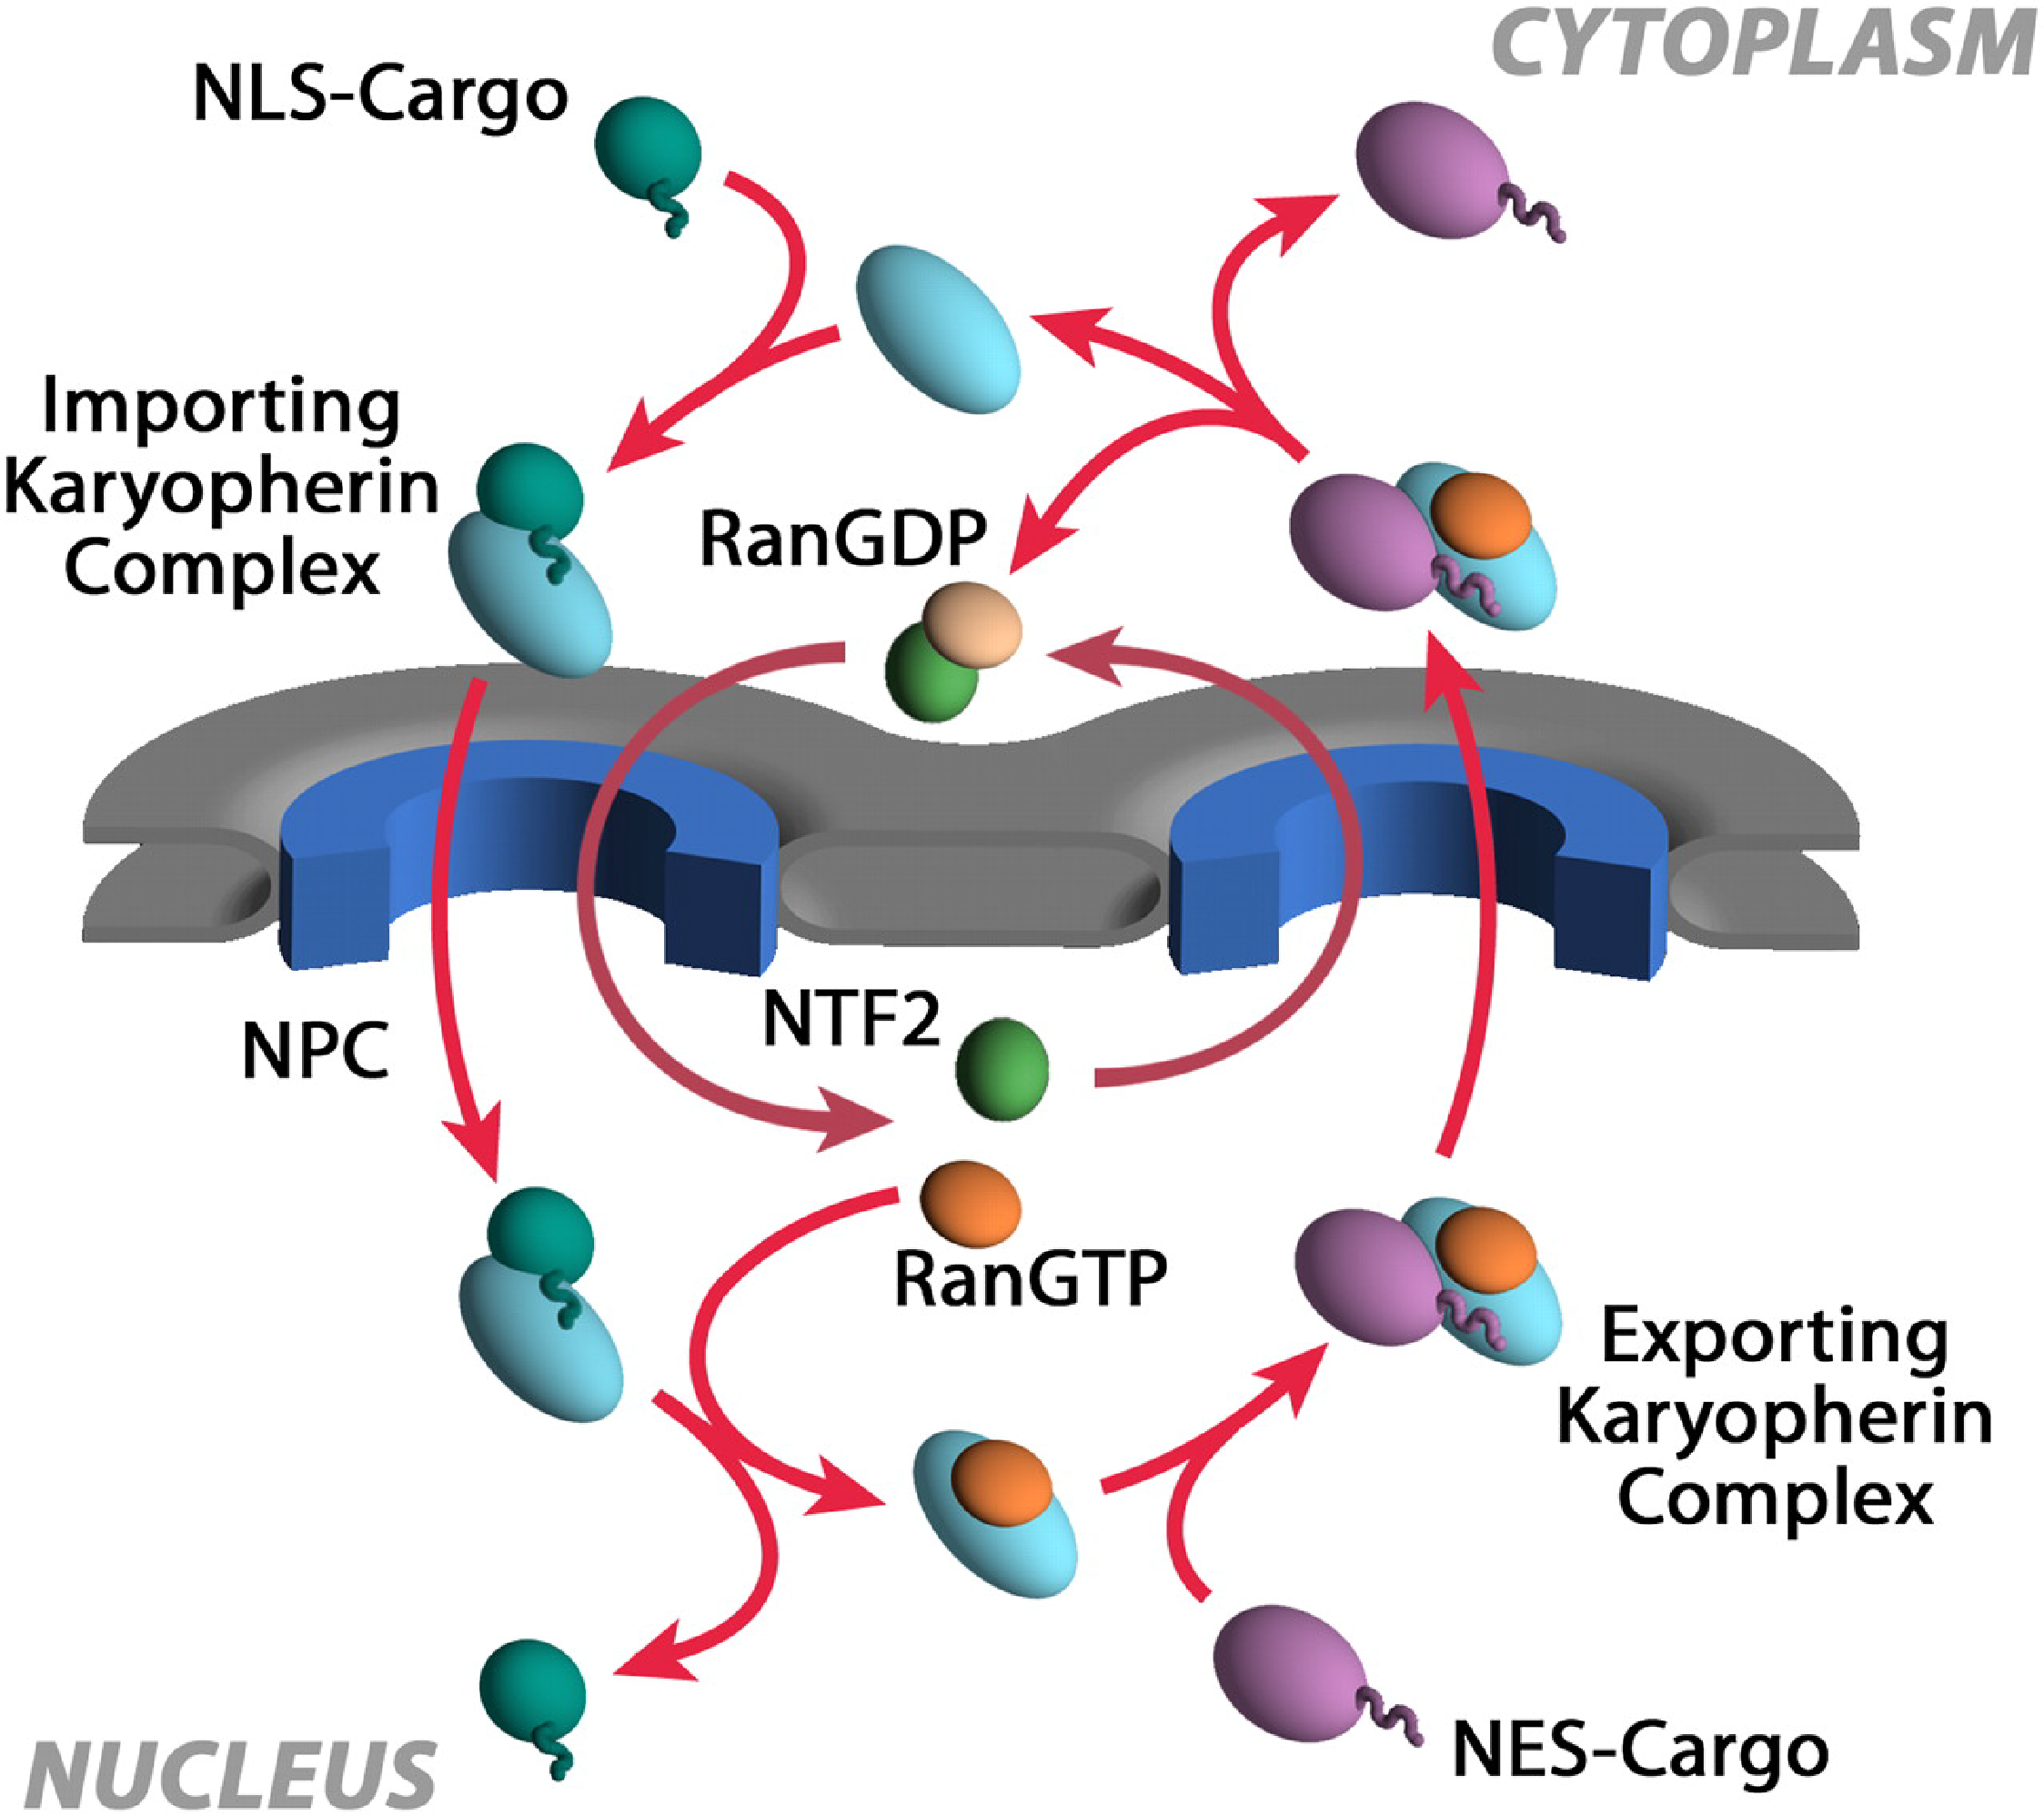
\includegraphics[width=0.65\linewidth]{figures/Figure1.4.pdf}
	\caption{Schematic of the RanGTP-regulated nuclear transport and their cargoes. Adapted from \cite{Aitchison2012}.}
	\label{fig:fig1.4}
\end{figure}

\subsection{Models of selective transport }
While nucleocytoplasmic transport is well characterized in terms of key players and regulation processes, the exact mechanism governing the selective transportation of cargo-bound NTRs through the NPC channel is still disputed. In fact, a number of models have been proposed which can be broadly classified into two opposing theories, termed ‘FG-centric’ and ‘Kap-centric’ models:\\[0.3pt]

\noindent\textbf{FG-centric models}: The first class of models includes the ‘virtual gate model’\cite{Rout2003}, ‘selective-phase’ or ‘hydrogel model’ \cite{Frey2006,Frey2007}, and ‘forest model’ \cite{Yamada2010}, which predict that FG-Nups are the sole necessary ingredient in establishing the selective barrier. As a corollary, this implies that Kaps act as mere transporters of cargo molecules, without in any way altering the structure of the FG-mesh or taking part into forming the selective barrier (Fig.\ref{fig:fig1.5}, left).

\begin{figure}[!htbp]
	\centering
	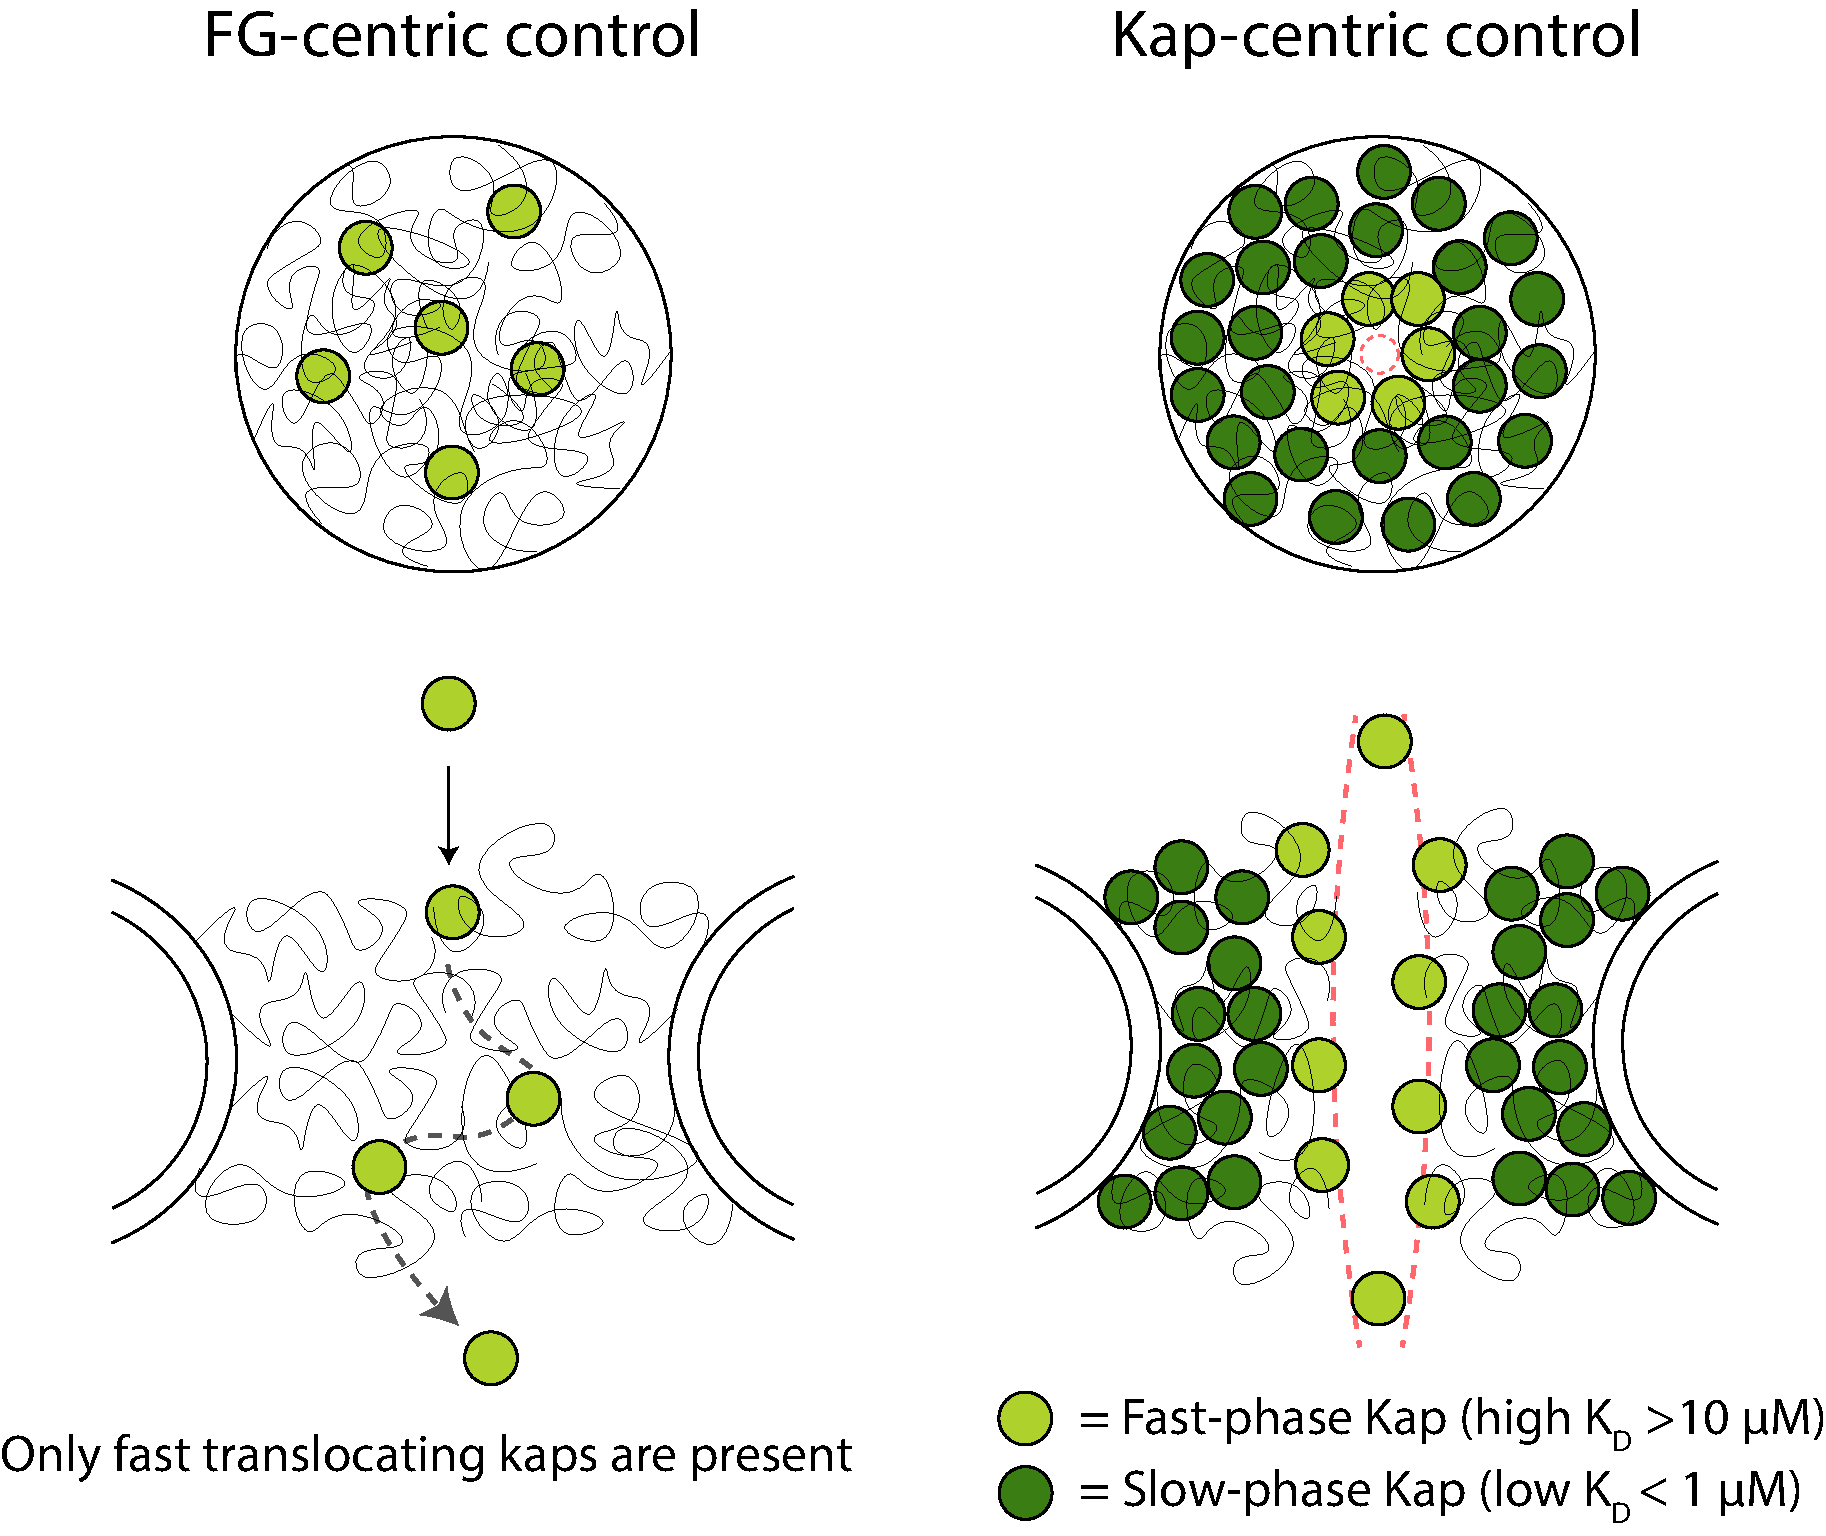
\includegraphics[width=1\linewidth]{figures/Figure1.5.pdf}
	\caption{Simplified schematic of ‘FG-centric’ (left) and ‘Kap-centric’ (right) transport. Black curved lines represent FG-Nups, light and dark green circles correspond to the fast-phase and slow-phase Kap population, respectively, dashed black arrow (left) represent a Kap trajectory, dashed red lines (right) indicate the central channel opening. Inspired by \cite{Kapinos2014} and \cite{Kapinos2017a}.}
	\label{fig:fig1.5}
\end{figure}
\newpage
\noindent\textbf{Kap-centric models}: The second class of models, such as the ‘reduction of dimensionality model’ \cite{Peters2005}, ‘molecular velcro model’ \cite{Schleicher2014}, and further refinements \cite{Kapinos2014,Lim2015,Wagner2015,Kapinos2017a,Barbato*2020}, supports the existence of two distinct populations of Kaps – a ‘slow-phase’ and a ‘fast-phase’, where the slow-phase Kaps are involved in reshaping the FG-mesh while opening a central channel by means of avid multivalent binding to FG-repeats, whereas fast-phase Kaps are the actual transporters that shuttle the cargo across the NPC (Fig.\ref{fig:fig1.5}, right).  Importantly, occupation of the FG-mesh by the slow-phase Kaps would result in a partial depletion of the available FG-repeats hence lowering the affinity between the Kap-laden FG-mesh and the fast-phase Kaps.

\section[Bottom-up approaches to unravel the NPC]{Bottom-up approaches to unravel the NPC}
\sectionmark{Chapter 1}
Studying transport through the nuclear pore complex \emph{in vivo} still faces significant challenges and limitations due to a lack of spatiotemporal resolution. The NPC is a complex machine, comprising $\sim$200 intrinsically disordered FG-Nups confined into a $\sim$40nm-wide central lumen, with $\sim$1000 molecules per second being transported across in both directions \cite{Jamali2011}. Gaining mechanistic information on the translocation process of Kap-cargo complexes through the FG-mesh has thus far remained prohibitively difficult. 

To overcome such challenges, biomimetic techniques have emerged as an alternative approach to study nuclear transport, where the FG-mesh that is found in the central channel of the NPC is reconstituted \emph{in vitro} and characterized using a variety of tools. Notable examples include surface techniques, such as ellipsometry and QCM-D \cite{Eisele2010a,Eisele2013a}, SPR \cite{Schoch2012,Kapinos2014}, and AFM force spectroscopy \cite{Lim2007,Schleicher2014}, which contributed greatly to the characterization of the binding affinity between Kaps and FG-Nup brushes, where such brushes were formed by anchoring FG-Nups to a planar surface with a grafting density comparable to the one found in the real NPC. Importantly, such techniques revealed the presence of distinct binding modes between Kaps and FG-Nup brushes that vary as a function of Kap concentration and that stem from the multivalent nature of the interaction.

While studying the affinity between transporters and FG-Nups is beneficial and insightful, selective transmembrane transport is arguably the most crucial, yet puzzling, feature of the NPC. To study such important aspect, in the last decade NPC mimics based on artificial nanopores have been built by tethering purified FG-Nups to the inner walls of a nanopore \cite{Jovanovic-Talisman2009,Kowalczyk2011a}. The appeal of this approach resides in the possibility to reconstitute the selective FG-Nup barrier into a confined nanopore system with virtually the same geometry and FG-Nup density as the NPC central channel. We will now introduce two major realizations of biomimetic nanopores that take advantage of state-of-the-art solid-state and DNA-origami nanotechnology. 


\section[Single-molecule sensing with nanopores]{Single-molecule sensing with nanopores}
\sectionmark{Chapter 1}
Advancements in nanotechnology have enabled the fabrication and development of solid-state nanopores \cite{Dekker2007,Xue2020}. In simple terms, a solid-state nanopore can be described as a nanometer-sized hole formed across a thin (typically $\sim$20 nm) freestanding membrane built from a solid-state material. Over the years, a variety of membranes have been employed as substrates for nanopore fabrication, from the more common low stress silicon nitride \cite{Balan2014,Venta2013}(SiN) to silicon dioxide (SiO\textsubscript{2}), as well as ultrathin 2D-materials such as graphene \cite{Merchant2010,Schneider2010}, hexagonal boron nitride (hBN)\cite{Zhou2013,Park2016}, or molybdenum disulfide (MoS\textsubscript{2}) \cite{Graf2019}. To create such nanoholes various techniques have been developed that respond to different needs in terms of precision, cost, and throughput. To create pores with nanometer-precision a transmission electron microscope (TEM) is usually the preferred choice (Fig.\ref{fig:fig1.6}a,b), where a beam of electrons is focused onto a freestanding membrane which results in removal of atoms from the material and the formation of a hole \cite{Storm2003}. A more high-throughput, though less precise, method to fabricate pores is milling using a focused ion beam (FIB) \cite{Lanyon2007,Schiedt2010}, which works analogously to the TEM but with ions (typically Ga\textsuperscript{+} or He\textsuperscript{+}) instead of electrons. Other techniques are dielectric breakdown \cite{Kwok2014,Pud2015}, laser etching \cite{Gilboa2019}, reactive ion etching (RIE) \cite{Verschueren2018}, and mechanical pulling of glass capillaries \cite{Piper2006}. 

The most common application of nanopore technology consists in single-molecule sensing, which is achieved by encasing the nanopore chip in a flow cell where the nanopo\-re constitutes the sole connection between two otherwise insulated compartments \cite{Maglia2010}. Such compartments are filled with a saline aqueous solution, \emph{e.g.} potassium chloride (KCl), which results in free K\textsuperscript{+} and Cl\textsuperscript{-} ions. Application of a voltage difference across the freestanding membrane results in an electric field across the pore that drives positive ions K\textsuperscript{+} to the side with negative potential and Cl\textsuperscript{-} to the positive one. Such flow of ions across the pore results in an ionic current which can be sensed by the electronics and that serves as the signal to perform sensing \cite{Howorka2009}. 

The basic principle of nanopore sensing is illustrated in Figure \ref{fig:fig1.6}c,d, where the analyte of interest, such as a protein or a DNA molecule, is electrophoretically driven across the pore by the applied voltage difference which causes the flow of ions to be temporarily interrupted due to the presence of the molecule. This effectively results in a transient, detectable decrease of the ionic current (Fig.\ref{fig:fig1.6}d). Single-molecule translocation events are associated with such current ‘spikes’ and are typically characterized in terms of amplitude (or blockade), 
\begin{figure}[!htbp]
	\centering
	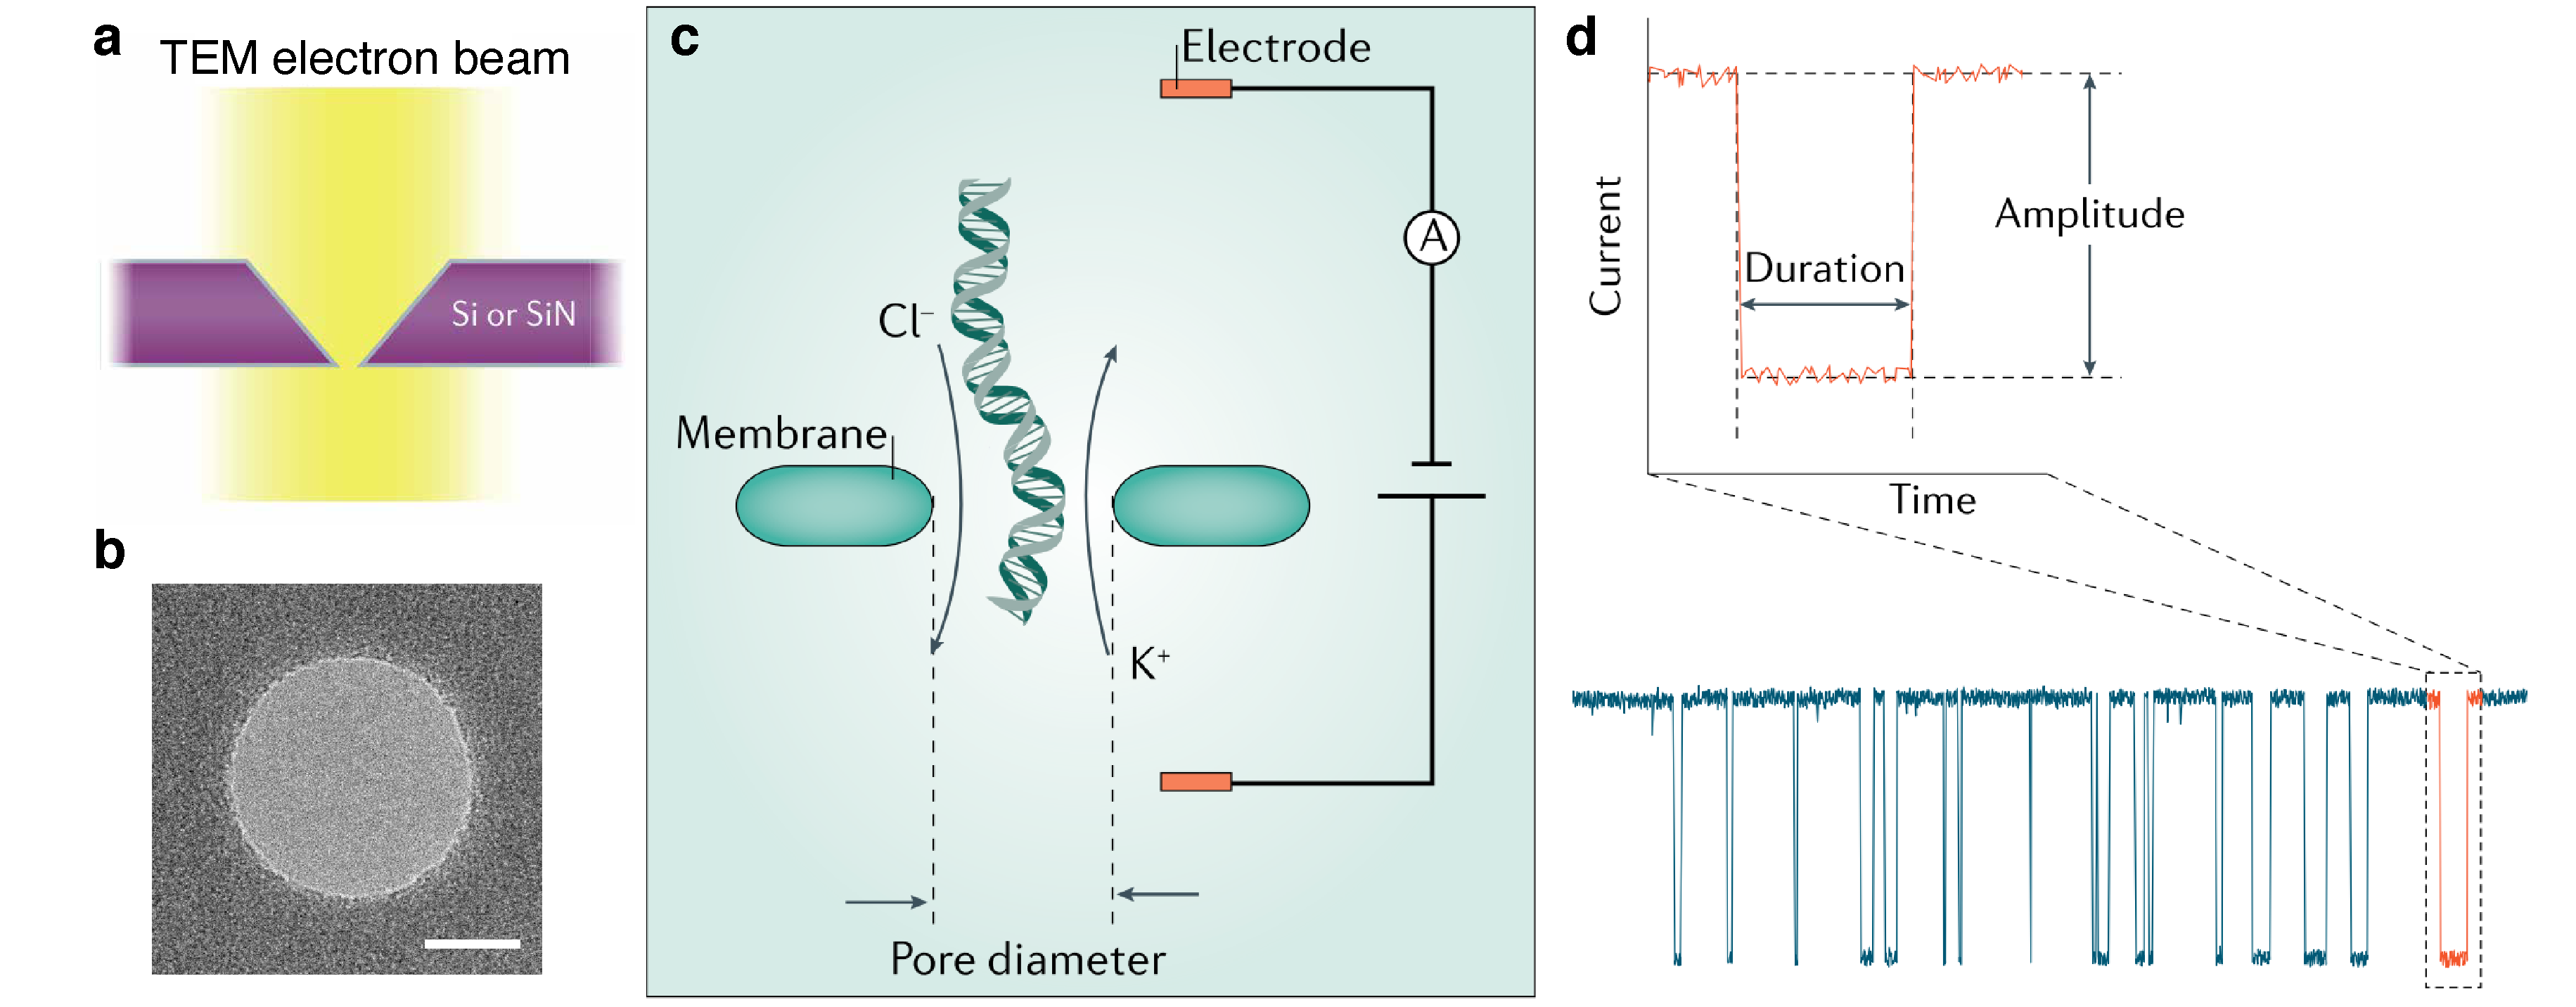
\includegraphics[width=1\linewidth]{figures/Figure1.6.pdf}
	\caption{a, Illustration of nanopore fabrication by TEM drilling. b, TEM micrograph of a nanopore. Scale bar, 30nm. c–d Principle of nanopore sensing: molecules are electrically driven through the pore by an applied potential difference causing transient dips (d) in the ionic current. a, c, d, were adapted from \cite{Xue2020}.}
	\label{fig:fig1.6}
\end{figure}
namely the depth of the current decrease which is roughly proportional to the size of the analyte, and dwell time which corresponds to the duration of the event and, to a first approximation, reflects how much time the molecule spends in the pore.

\subsection{Biomimetic solid-state nanopores}
While nanopores are usually thought of as next-generation sequencers of DNA \cite{Manrao2010} and proteins \cite{Brinkerhoff2021}, an exciting application consists in mimicking biological processes by recapitulating the behavior of naturally occurring pores such as the NPC. In the context of this thesis, a biomimetic solid-state nanopore consists of a solid-state nanopore that is functionalized with FG-nucleoporins from the nuclear pore complex with the aim to mimic as closely as possible the native FG-mesh in terms of spatial confinement, geometry, and protein density, while being able to probe the transport across the pore with single-molecule resolution by measuring the ionic current (Fig.\ref{fig:fig1.7}a). Functionalization of the nanopore surface is generally carried out by a chemical conjugation protocol \cite{Kowalczyk2011a,Ananth2018}, which ensures proper covalent attachment of the proteins to the solid-state material. To test the selective properties of the reconstituted FG-mesh, transporter proteins, such as Imp$\beta$, are used as positive control since they are naturally capable of interacting with and overcoming the FG-Nup barrier. On the contrary, inert proteins like BSA that lack binding sites for FG-repeats are repelled by the FG-mesh and thereby fail to traverse the pore. 

Current measurements are carried out similarly as in a standard nanopore experiment, where the current flowing across the FG-Nup-coated pore reports in real-time on the passage of proteins (Fig\ref{fig:fig1.7}b), and thus allows to assess the selective transport properties in terms of event rate, \emph{i.e.} number of translocations per second, which is a measure of the transport efficiency of the analyte across the pore. Notably, such current measurements revealed that biomimetic pores built using a single type of FG-Nup (\emph{e.g.}, Nup98 or Nup153) were enough to impart a selective barrier, where Imp$\beta$ can efficiently translocate while BSA is blocked (Fig.\ref{fig:fig1.7}c) \cite{Jovanovic-Talisman2009,Kowalczyk2011a,Ananth2018}.
\begin{figure}[!htbp]
	\centering
	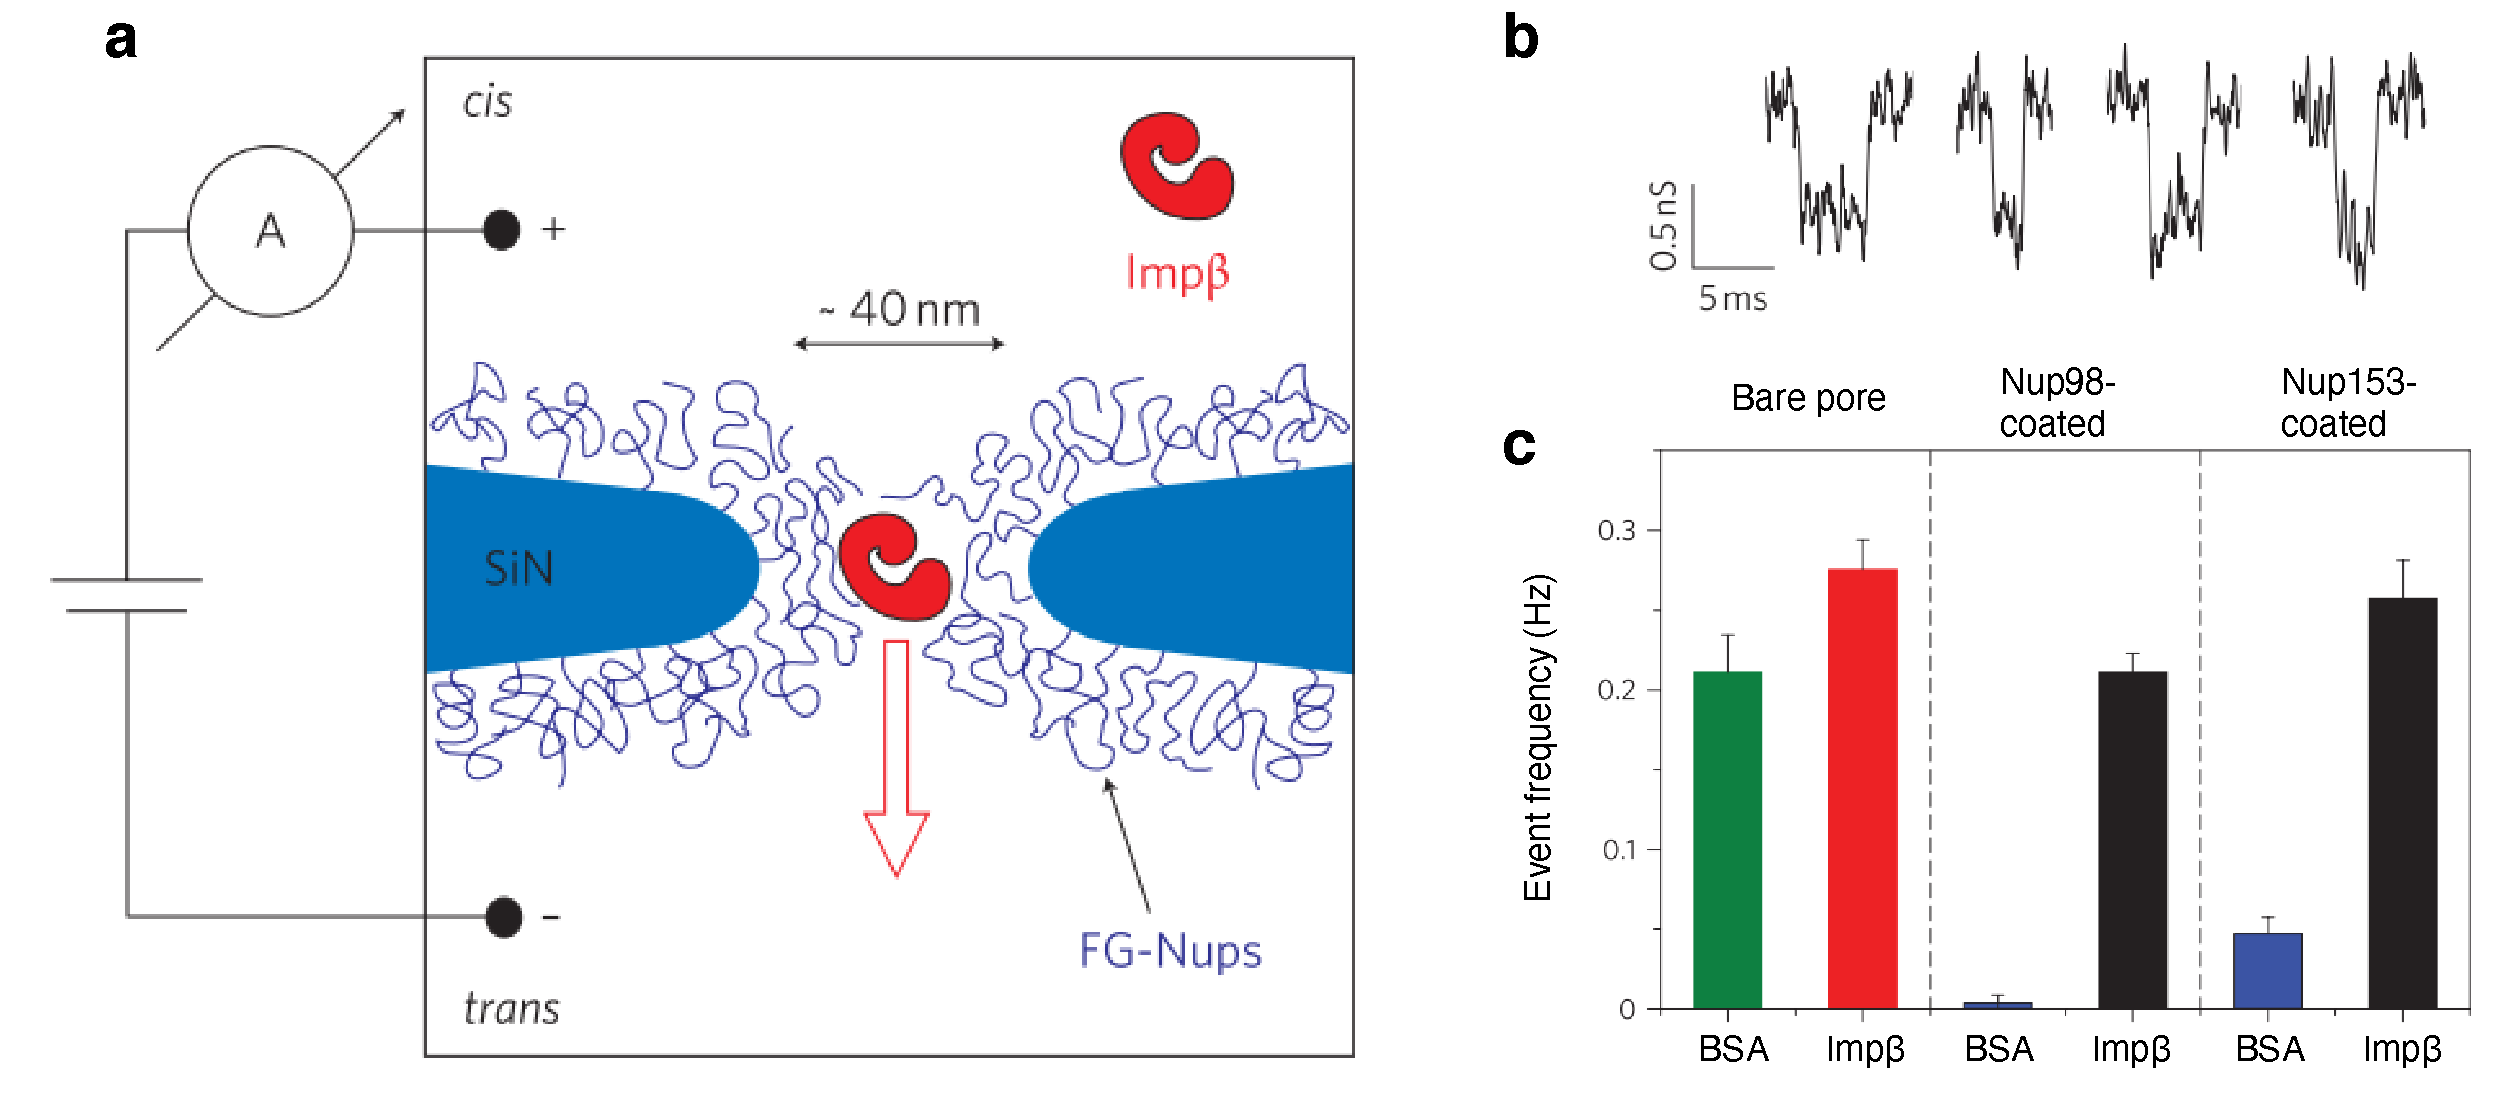
\includegraphics[width=0.95\linewidth]{figures/Figure1.7.pdf}
	\caption{a, Schematic of a biomimetic solid-state nanopore system. b, Examples of translocation events of Imp$\beta$ through a FG-Nup coated pore. c, Event rate of translocations of BSA and Imp$\beta$ through a bare (left), Nup98-coated (center), and Nup153-coated (right) pores. Adapted from \cite{Kowalczyk2011a}.}
	\label{fig:fig1.7}
\end{figure}

\section[DNA origami nanotechnology]{DNA origami nanotechnology}
\sectionmark{Chapter 1}
While DNA (deoxyribonucleic acid) in biology assumes the passive role of mere information carrier, as unlike proteins it does not perform any sensory or actuatory function in the cell, in the last three decades scientists have been able to use DNA molecules to build 3D nanostructures from scratch in a fully programmable way \cite{Rothemund2006,Wagenbauer2017a}. Such promising technology, known as ‘DNA origami’, exploits the structure of the DNA molecule that consists of two strands of nitrogenous bases (adenine (A), guanine (G), thymine (T), and cytosine (C)) that are mutually held together by hydrogen bonds resulting in a double helix, where such bonds can occur only between complementary bases A-T and G-C. 

Creation of DNA nanostructures relies on using a long single strand of DNA as a scaffold which, upon adding many short DNA strands that staple different parts of the scaffold, is folded into a 3D shape (Fig \ref{fig:fig1.8}a) \cite{Sanderson2010}. Using this relatively simple concept it has been possible to build a multitude of nanostructure for various purposes, from regular shapes such as 2D-sheets and cubes (Fig.\ref{fig:fig1.8}b) \cite{Rothemund2006}, to more complex structures such as spirals and rings (Fig.\ref{fig:fig1.8}c) \cite{Dietz2009}.



\begin{figure}[!htbp]
	\centering
	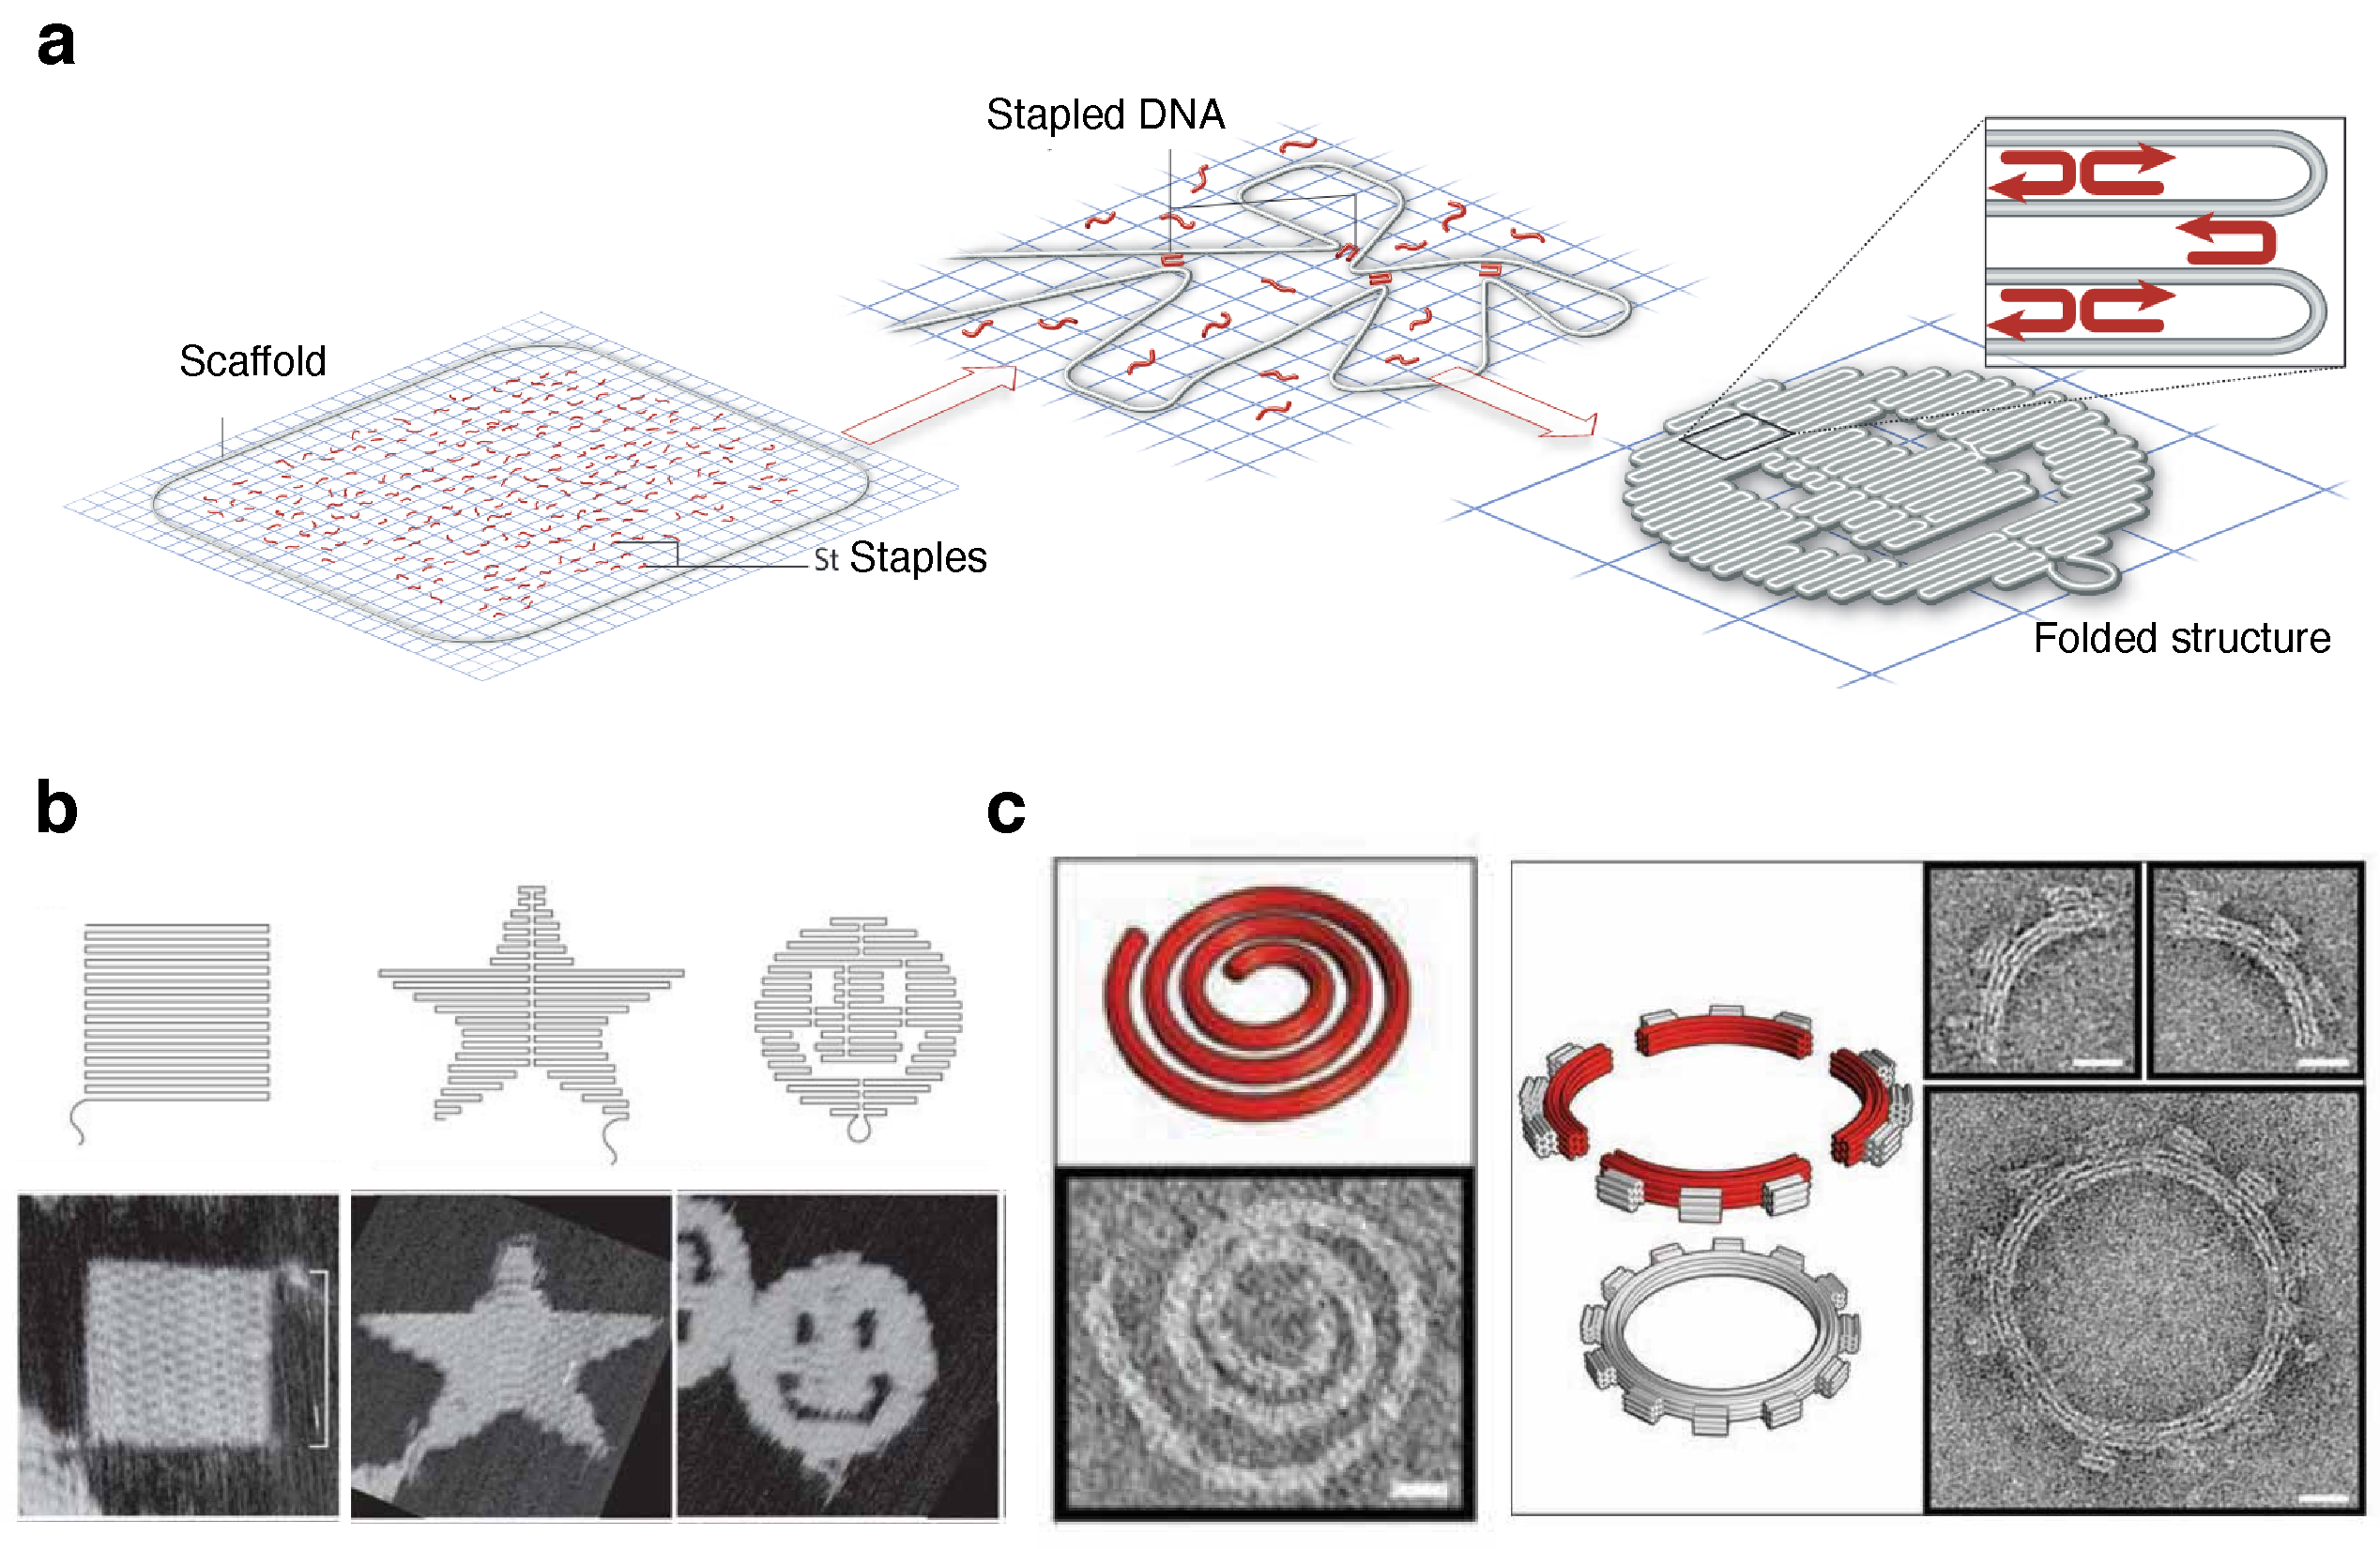
\includegraphics[width=1\linewidth]{figures/Figure1.8.pdf}
	\caption{a, Illustration of the typical DNA origami workflow. A long scaffold of DNA is stapled together by short pieces of DNA to form a stably folded structure. Adapted from \cite{Sanderson2010}. b, Examples of design (top) and AFM images (bottom) of simple DNA-origami structures. Adapted from \cite{Rothemund2006}. c, Examples of complex twisted DNA-origami structures. Scale bars, 20nm. Adapted from \cite{Dietz2009}.}
	\label{fig:fig1.8}
\end{figure}
\newpage
\subsection{DNA origami nanopores and NPC mimics}
A relevant application in the context of this thesis is the construction of DNA-origami pores that mimic the pore-forming properties of naturally occurring protein pores such as $\alpha$-hemolysin \cite{Sugawara2015}. Similarly to a biological pore, DNA-origami pores from the literature have been engineered with hydrophobic moieties, such as cholesterols or porphyrins, that aid in the insertion of the highly hydrophilic DNA-object into a lipid bilayer membrane (Fig.1.9) \cite{Hernandez-Ainsa2014}. Using this approach, pores with inner diameters from a few nanometers \cite{Martin2012,Burns2016} up to 10 nm \cite{Thomsen2019,Iwabuchi2021} have been constructed and shown to spontaneously insert into a lipid membrane by allowing the transmembrane transport of ions \cite{Martin2012,Gopfrich2016}, fluorophores \cite{Krishnan2016,Thomsen2019}, and short artificial polymers such as PEG \cite{Burns2016} and dextran \cite{Thomsen2019,Iwabuchi2021}. 


An exciting feature of DNA-origami pores is the possibility to functionalize the inner walls of the pore to build a mimic of the NPC where FG-Nups distribution and density of the anchor points can be programmed by design. Using this approach, it has been possible to reconstitute NPC mimics by folding DNA-origami rings of $\sim$35-40 nm in inner diameter (similar to the native NPC) and by attaching FG-Nups to their inner surface \cite{Ketterer2018,Fisher2018}. However, one major limitation of this approach is the impossibility to measure transport across the reconstituted FG-mesh, since it is extremely challenging to insert such large DNA-objects into a lipid bilayer.

\begin{figure}[!htbp]
	\centering
	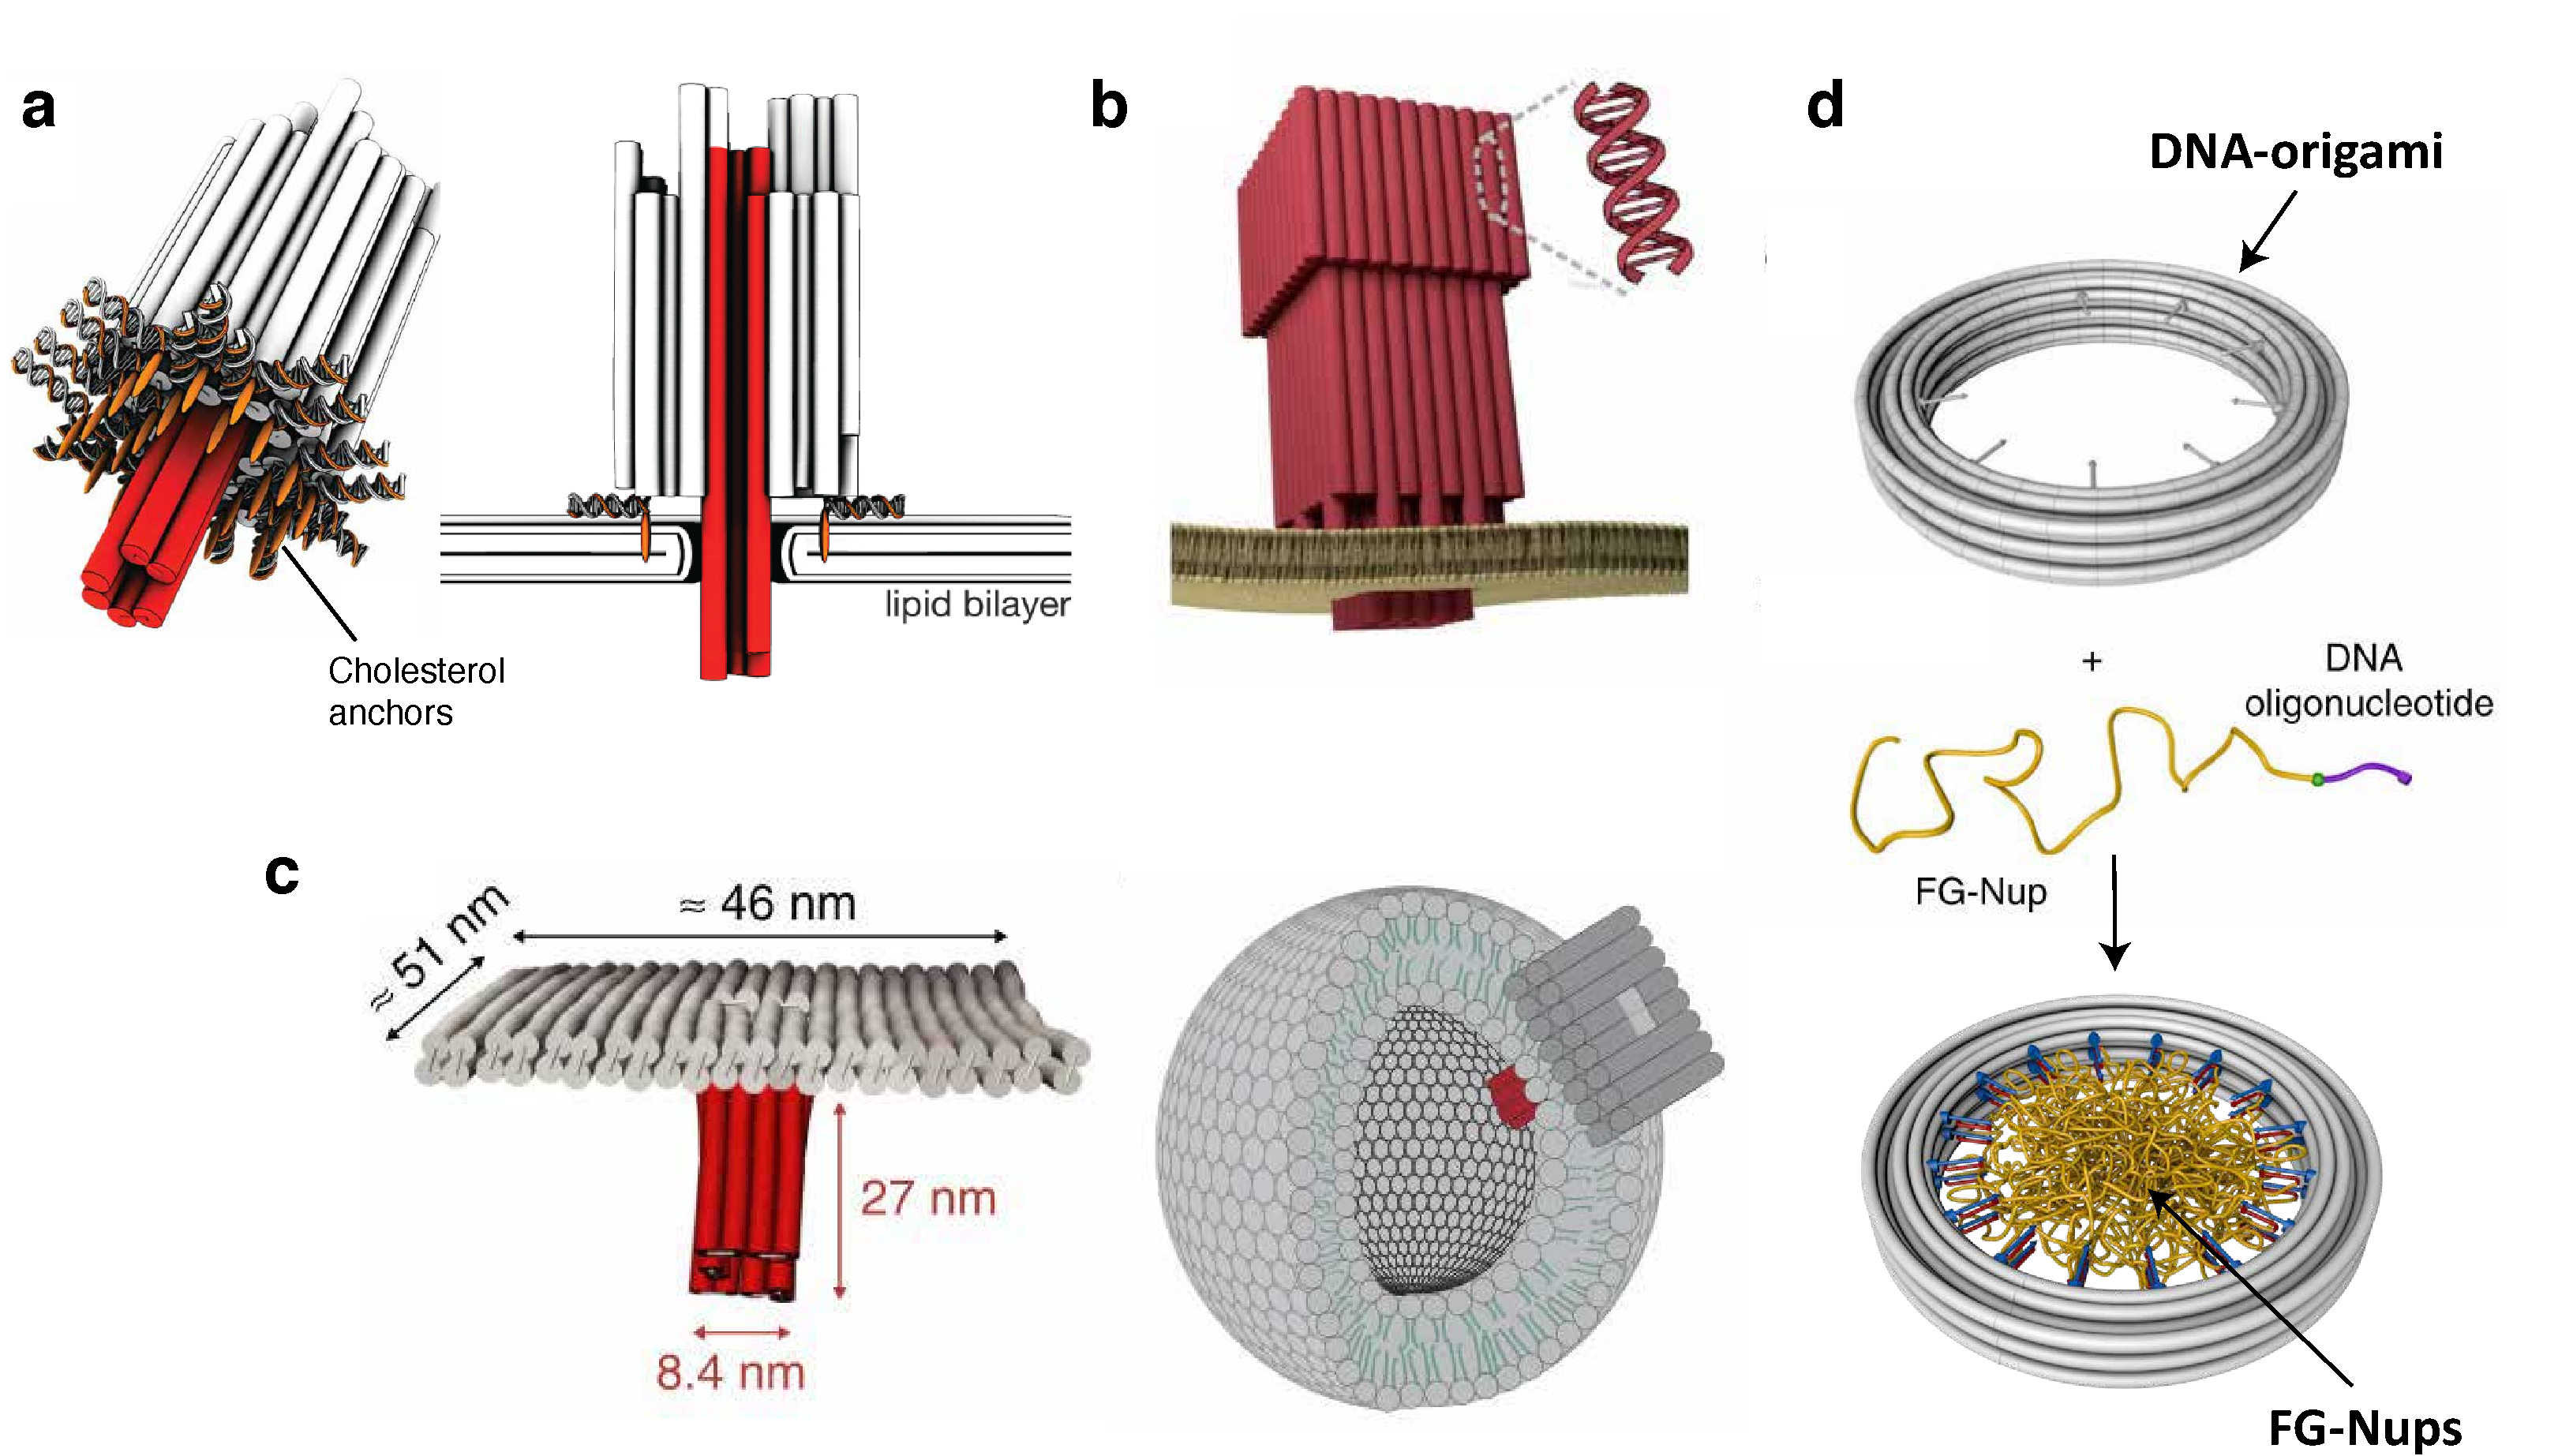
\includegraphics[width=1\linewidth]{figures/Figure1.9.pdf}
	\caption{a, First reported DNA-origami pore with a inner diameter of 2 nm, functionalized with 26 cholesterol anchors (orange). Adapted from \cite{Martin2012}. b, Funnel-shaped transmembrane DNA-pore with 6 nm inner diameter. Adapted from \cite{Gopfrich2016}. c, T-shaped DNA-origami pore with $\sim$4 nm inner diameter. Adapted from \cite{Krishnan2016}. d, DNA-origami ring scaffold (grey) for FG-Nup (yellow) attachment. Adapted from \cite{Ketterer2018}.}
	\label{fig:fig1.9}
\end{figure}



\newpage
%\section[middling version]{verbose version%
%	\sectionmark{terse version}}
%\sectionmark{terse version}

\section[In this thesis]{In this thesis%
\sectionmark{Chapter 1}}
\sectionmark{Chapter 1}
This thesis aims to contribute with novel bottom-up approaches to the field of nuclear transport using biomimetic nanopores. We propose a new model system to understand and capture the essence of FG-Nups, as well as alternative strategies to circumvent the current technical difficulties in current biomimetic DNA-origami nanopore systems. The next two chapters following the introduction are focused on characterization of the noise sources in solid-state nanopores. \textbf{Chapter 2}, provides a side-by-side comparison of the noise and performance of biological and solid-state pores. First, the physical origin of the noise at different frequencies is provided together with literature studies and measurements on a few exemplary nanopore systems. Second, the performance of the most relevant biological and solid-state nanopores is compared in terms of signal-to-noise ratio (SNR). We find that SiN\textsubscript{x} pores offer the highest SNR of $\sim$37 when measuring free translocations of short DNA homopolymers through the pores. Introducing a slowdown mechanism using a DNA-translocating motor protein on top of a MspA pore was shown to boost the SNR by >160-fold. Finally, we review reported methods from the literature that were shown to lower the noise for various nanopore systems and frequency ranges. In \textbf{Chapter 3}, we explore the low-frequency 1/f noise in solid-state nanopores for varying pore diameters and find that the 1/f noise magnitude decreases for increasing diameter of the pore. To capture this behavior, we build a generalized version of the previously proposed Hooge’s model for nanopores that includes explicit contributions from access region and pore surface. Additionally, we define different Hooge parameters for bulk and surface 1/f noise, which represent different mechanisms of fluctuations affecting the ionic current. Such model refinement allows for a more accurate characterization of the 1/f noise in solid-state nanopore systems.  \textbf{Chapter 4} reviews the state-of-the-art in the field of nanopores, with particular emphasis on applications beyond sequencing. These include single-molecule proteomics, biomarker detection by single-molecule liquid biopsy, pore nanoreactors to confine and study the chemistry of single polymers, and biomimetic nanopore-based approaches to study biological questions. 
\\[0.5pt]

\noindent In \textbf{Chapter 5} we introduce a novel, fully bottom-up approach to study nuclear transport by designing an artificial protein, termed ‘NupX’, that mimics and models native FG-Nups. To design such sequence, we proceed by first analyzing the properties of the naturally occurring GLFG-Nups from yeast. We hypothesize that a finite set of properties characteristic of GLFG-Nups is sufficient for recapitulating their selective behavior, namely: (i) regularly spaced FG and GLFG repeats, (ii) a bimodal distribution of amino acids forming a repulsive and a cohesive domain, and (iii) intrinsic disorder of the amino acid sequence. We first assess the affinity between brushes of our designer NupX and transporter Kap95 using QCM-D, finding that Kap95 binds the protein brush in a concen\-tration-dependent manner. On the contrary, flushing the inert protein BSA does not result in any detectable interaction, thereby proving the binding specificity between Kap95 and NupX. Next, we reconstitute NupX in biomimetic nanopores and test its selective properties, finding that while Kap95 can efficiently translocate through the pore resulting in frequent current spikes, BSA is blocked. Our experiments are complemented by molecular dynamics simulations which provide insights into microscopic features of NupX brushes and coated pores. In summary, this work validates our initial hypothesis that a rationally designed FG-Nup can reconstitute the archetypal selectivity of the nuclear pore complex.
\\[0.5pt]

\noindent In \textbf{Chapter 6} we reconstitute biomimetic solid-state nanopores using a native FG-Nup, Nsp1, and test its transport properties as a function of Kap95 concentration with the aim to provide new evidence that can aid to discriminate between the different models of transport, specifically between ‘FG-centric’ and ‘Kap-centric’ models. Upon titrating Kap95 onto a Nsp1-coated pore we observe a Kap95 concentration-dependent step-wise decrease of the pore conductance, which indicates Kap95 incorporation into the Nsp1-mesh. Additionally, fast Kap translocations are also observed on top of the current decrease at low ($\sim$100 nM) Kap concentrations, similarly to previous reports. On the contrary, flushing inert BSA on a Nsp1-coated pore at increasing concentrations did not result in any detectable current decrease, nor fast translocations, confirming that the observed incorporation of Kap95 into the Nsp1-mesh originates from specific protein-protein interactions and not merely as an effect of the applied bias. Next to a decrease in the pore conductance, we also report a decrease of the low-frequency 1/f noise which is consistent with a stiffening of the Nsp1-mesh upon binding of Kap95. Ion current measurements are corroborated with QCM-D data that, similarly, show a concentration-dependent binding and incorporation of Kap95 into the Nsp1 brush. Altogether, our data are consistent with the ‘slow-phase’ and ‘fast-phase’ Kaps notions introduced by the Kap-centric models.
\\[0.1cm]

\noindent \textbf{Chapter 7} provides an alternative approach to solve the current challenges faced by DNA-origami nanopore systems, namely the difficulty of inserting large DNA-origami objects into lipid membranes. To mimic the eight-fold symmetry and geometry of the NPC, we first design an octagonal DNA-origami scaffold with a nominal inner diameter of 35 nm. Next, we chemically decorate its external surface with hydrophobic moieties which are meant to facilitate the partitioning of the DNA-origami structure into the hydrophobic lipid bilayer. We show that, while DNA-pores do not spontaneously insert into pre-formed lipid bilayers, as expected given the large size, it is possible to circumvent this problem by administering the pores during the vesicle formation by employing an inverted-emulsion cDICE technique to produce the vesicles. To assess the correct insertion of the pores, we carry out influx experiments with the fluorescent protein GFP and find that $\sim$50\% of the vesicle population features open pores. We quantify the influx rate by using a FRAP assay and, using a diffusion model to fit the FRAP data, find that up to hundreds of pores can be properly reconstituted into the membrane of a single vesicle. Furthermore, we show that our pores are size-selective, since dextran molecules with sizes up 28 nm can translocate the pores, whereas larger molecules are excluded.

\noindent In \textbf{Chapter 8}, finally, I provide my perspective on future possible directions and key experiments aimed to address some major open questions in the field of nuclear transport.


%% Start the actual chapter on a new page.
\newpage



\references{chapter-1/chapter-1}

